
\documentclass[11pt]{article}

%\setlength\topmargin{-0.1in}
%\setlength\headheight{0in}
%\setlength\headsep{0in}
\setlength\textheight{8.5in}
\setlength\textwidth{6.5in}
\setlength\oddsidemargin{0in}
\setlength\evensidemargin{0in}
\setlength{\parindent}{0pt}
\usepackage{placeins}
%\usepackage{indentfirst}

\usepackage{amsmath}
\usepackage{graphicx}
\usepackage{listings}
\usepackage{rotating}
\usepackage{subcaption} 
\usepackage{booktabs}
\usepackage{tikz}
\usepackage{fancyhdr}
\usepackage{pdfpages}
\usepackage{hyperref}
\usepackage{longtable}
\usepackage[toc,page]{appendix}
%For The 2x2 Figure
\usepackage{subcaption}
\usepackage{mwe}
%Put table captions above
\usepackage{floatrow}
\floatsetup[table]{capposition=top}
% To import matlab code
\usepackage{listings}
\usepackage{matlab-prettifier}
\usepackage[framed,numbered,autolinebreaks,useliterate]{mcode}
%Glossary
\usepackage[acronym,nonumberlist]{glossaries}
%\glsaddall %includes all acronymns
%Tables
\usepackage{booktabs}
\newcommand{\ra}[1]{\renewcommand{\arraystretch}{#1}}
%Nomenclature
\usepackage{nomencl}
\makenomenclature
\newif\iffirstglossary\firstglossarytrue
%% This removes the main title:
\renewcommand{\nomname}{}
%% this modifies item separation:
\setlength{\nomitemsep}{15pt}
%% this part defines the groups:
%----------------------------------------------
\usepackage{etoolbox}
\renewcommand\nomgroup[1]{%
  \item[\Large\bfseries
  \ifstrequal{#1}{N}{Nomenclature}{%
  \ifstrequal{#1}{A}{List of Abbreviations}{}}%
]\vspace{10pt}} % this is to add vertical space between the groups.
%----------------------------------------------



\pagestyle{fancy}
\usetikzlibrary{shapes,arrows}
\graphicspath{{Figures/}}
\newcommand{\tabitem}{~~\llap{\textbullet}~~}

\newcommand*{\MyIndent}{\hspace*{0.5cm}}%inerts tab in tables



 
\begin{document} 
\pagenumbering{gobble}

	\begin{titlepage}
	\thispagestyle{empty}
		\newcommand{\HRule}{\rule{\linewidth}{0.5mm}}	
		\center
		\LARGE 
		University of Bath\\
	 	Faculty of Engineering \& Design\\[1cm]	
		%textbf{\Large ME30313 Group Business & Design}\\
		\large
		Word count: 2174\\[0.5cm]
		{\large\today}\\[1cm]	
		\HRule\\[0.4cm]	
		{\LARGE \bfseries Systems Modelling \& Simulation Coursework 2}\\[0.3cm] 	
		\HRule\\[1cm]	
		\begin{minipage}{0.4\textwidth}
			\begin{flushleft}
				\large
				\textit{Supervisor}\\
				A. \textsc{Cookson}
			\end{flushleft}
		\end{minipage}
		~
		\begin{minipage}{0.4\textwidth}
			\begin{flushright}
				\large
				\textit{Assessor}\\
				
			\end{flushright}
		\end{minipage}\\[1.4cm]
		\large
		\textit{Author's Candidate Number}\\
		10838\\
		\vfill
		\includegraphics[width=0.4\textwidth]{UOB_Logo.png}\\
		\vfill 
	\end{titlepage}

%%% ACRONYMS %%

%%END OF ACRONYMS %%%


\thispagestyle{empty}




\tableofcontents
\thispagestyle{empty}
\listoffigures


\nomenclature[A]{CAD}{Computer Aided Design}


%\printnomenclature


\clearpage
\pagenumbering{arabic}
%\setcounter{page}{1}

\section{Part 1: Software Verification}
This paper is based on solving the transient diffusion-reaction equation given by equation \eqref{eq:MAIN}.


\begin{equation}\label{eq:MAIN}
\frac{\partial c}{\partial t}    = D\frac{\partial^2 c}{\partial x^2} + \lambda c + f
\end{equation}

A transient Diffusion-Reaction solver was developed to solve equation \eqref{eq:MAIN}. A flow chart showing how this solver works is available in Appendix \ref{ap:TRDS}. The local element matrices and vectors were all evaluated using Gaussian Quadrature. All functions for the solver are available in the appendices.

\subsection{Question 1a}
\subsubsection{Introduction}

A transient Diffusion-Reaction solver was developed and used to solve the specific transient equation give by equation \eqref{eq:q1a}. This is the same equation as \eqref{eq:MAIN} with $\lambda = 0$ and $f = 0$. 

\begin{equation} \label{eq:q1a}
\frac{\partial c}{\partial t}    = \frac{\partial^2 c}{\partial x^2}
\end{equation}

The equation is subject to the following domain, boundary conditions and initial conditions.

\begin{equation*}
\begin{split}
x &= [0,1] \\
t &= [0,1] \\
c(x,0) &= 0 \\
c(0,t) &= 0 \\
c(1,t) &= 1
\end{split}
\end{equation*}

The analytical solution of equation \eqref{eq:q1a} for the above conditions is given by equation \eqref{eq:q1aAnal}.

\begin{equation} \label{eq:q1aAnal}
c(x,t) = x + \frac{2}{\pi} \sum_{n=1}^{\infty} \frac{(-1)^n}{n} e^{-n^2\pi^2t}\text{sin}(n\pi x)
\end{equation}



A Crank-Nicolson time stepping scheme was used with the recommended time step of $\Delta t = .01$ and a 10 element mesh. The result produced using the finite element method is compared to the analytical solution for $ t = 0.01, \ 0.10, \ 0.20, \ 1$ as shown by Figure \ref{fig:q1a}. The FEM solver incorporates the option of quadratic basis functions and so this solution has been plotted in Figure \ref{fig:q1aquad} alongside the linear basis function solution shown in Figure \ref{fig:q1alin}. The difference between the quadratic and linear solutions is hardly noticeable in these plots and both provide a good approximation to the analytical solution. It is clear that the FEM solutions converge on the analytical solution as time increases with the plots indistinguishable at $t = 1$ where the steady state solution has been approached.

\begin{figure}[h!] 
        \centering
        \begin{subfigure}[b]{0.475\textwidth}
            \centering
            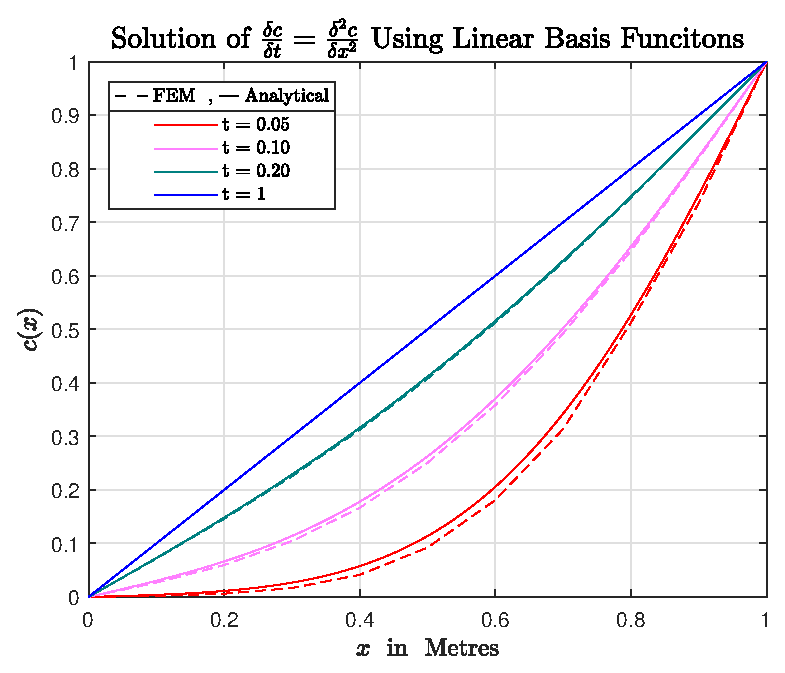
\includegraphics[width=\textwidth]{epsQ1a}
            \caption[]%
            {{\small Linear Basis Function Solution }}    
            \label{fig:q1alin}
        \end{subfigure}
        \hfill
        \begin{subfigure}[b]{0.475\textwidth}  
            \centering 
            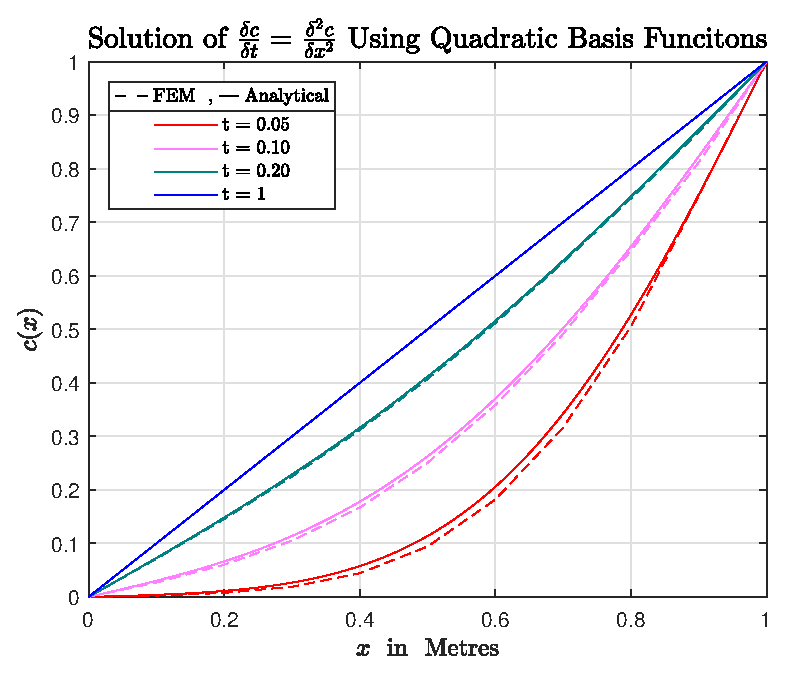
\includegraphics[width=\textwidth]{epsQ1aQuad}
            \caption[]%
            {{\small Quadratic Basis Function Solution}}    
            \label{fig:q1aquad}
        \end{subfigure}
        \caption[ Comparison of FEM and Analytical Results Over Spatial Domain ]
        {\small Comparison of FEM  and Analytical Results with 10 Elements for Linear, 5 Elements for Quadratic, Crank-Nicolson Time Stepping using $\Delta t = 0.01s$} 
        \label{fig:q1a}
\end{figure}

\FloatBarrier
\subsection{Question 1b}
The solution was also compared to the analytical solution across the time domain at $x = 0.8$ which can be seen in Figure \ref{fig:q1b}. The result generally compares well with the analytical solution with $c \rightarrow x $ as  $t \rightarrow \infty $. It is worth noting that the error is noticeable for small values of $t$ as shown in Figure \ref{fig:q1bzoom}. There is a 4\% error at $t = 0.051s$ due to the steep gradient at this point however by $t = 0.20s $ where the gradient has begun to reduce the error is less than 0.5\%. 



\begin{figure}[h!] 
        \centering
        \begin{subfigure}[b]{0.475\textwidth}
            \centering
            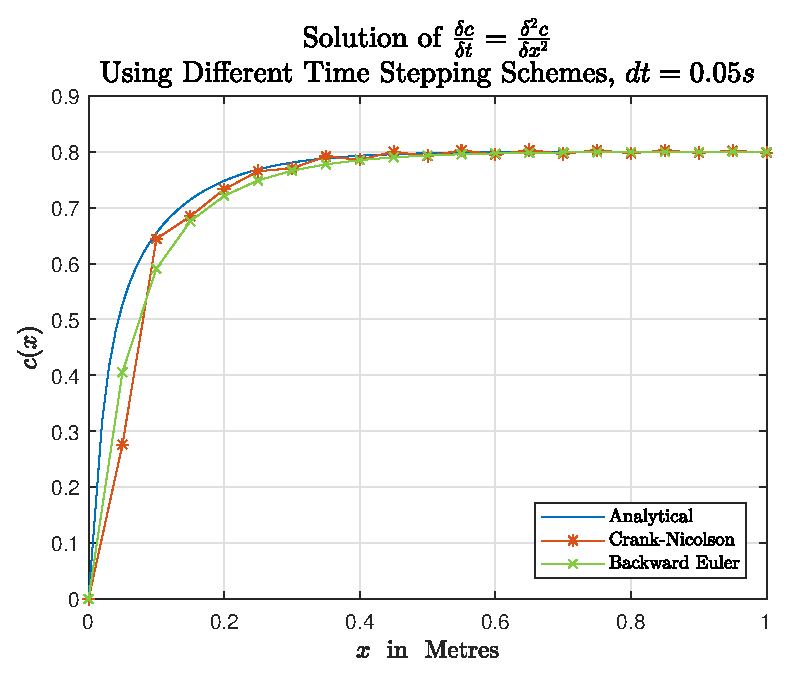
\includegraphics[width=\textwidth]{epsQ1b}
            \caption[]%
            {{\small Solution at x = 0.8m Over Time Domain }}    
            \label{fig:q1b}
        \end{subfigure}
        \hfill
        \begin{subfigure}[b]{0.475\textwidth}  
            \centering 
            \includegraphics[width=\textwidth]{epsQ1bZoom}
            \caption[]%
            {{\small Detailed Look at t = 0.05 to t = 0.051}}    
            \label{fig:q1bzoom}
        \end{subfigure}
        \caption[ Comparison of FEM and Analytical Results Over Spatial Domain at $x = 0.8m$]
        {\small Comparison of FEM and Analytical Results with Crank-Nicolson Time Stepping and 10 element Quadratic Basis Function Mesh.} 
        \label{fig:q1a}
\end{figure}

\FloatBarrier
\subsection{Investigation of Time Stepping Schemes}

The times stepping schemes used were Backward Euler and Crank-Nicolson. The results at $x = 0.8m$ for over the time range have been plotted for both time stepping schemes at time steps of $\Delta t = 0.10s$ and $\Delta t = 0.025s$ in Figures \ref{fig:q1b10} and \ref{fig:q1b025} respectively. With a time step of $\Delta t = 0.1s$  the Crank-Nicolson scheme is showing an oscillatory solution whereas the Backward Euler scheme does not oscillate. The oscillatory response of the Crank-Nicolson reduces with time and is more accurate over the time domain than the Backward Euler scheme, even at the larger 0.10s time step. As the time step is reduced to $\Delta t = 0.02s$ the oscillation of the Crank-Nicolson scheme is much less pronounced and is again visibly more accurate that the Backward Euler scheme. 

\begin{figure}[ht] 
        \centering
        \begin{subfigure}[b]{0.475\textwidth}
            \centering
            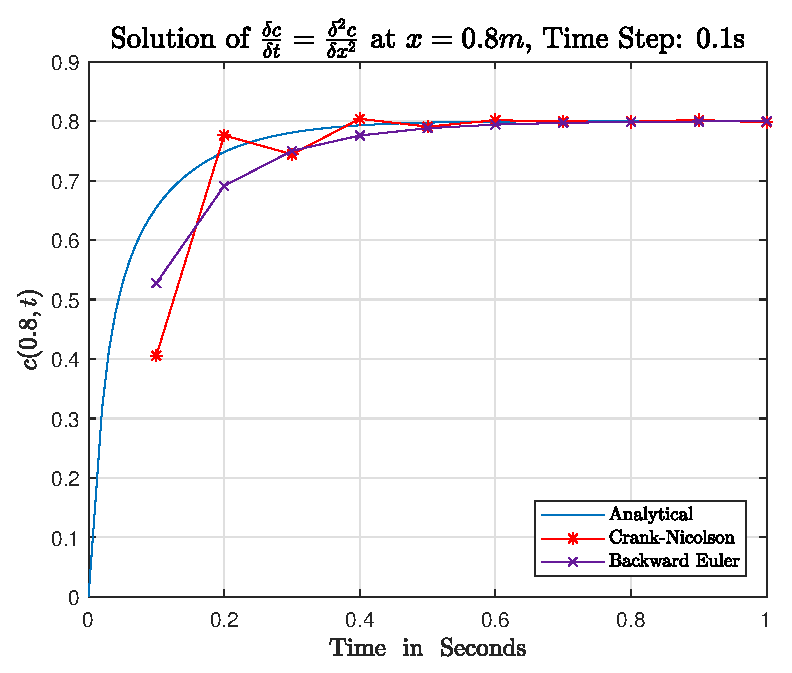
\includegraphics[width=\textwidth]{epsQ1bdt05}
            \caption[]%
            {{\small Time Step of 0.1s }}    
            \label{fig:q1b10}
        \end{subfigure}
        \hfill
        \begin{subfigure}[b]{0.475\textwidth}  
            \centering 
            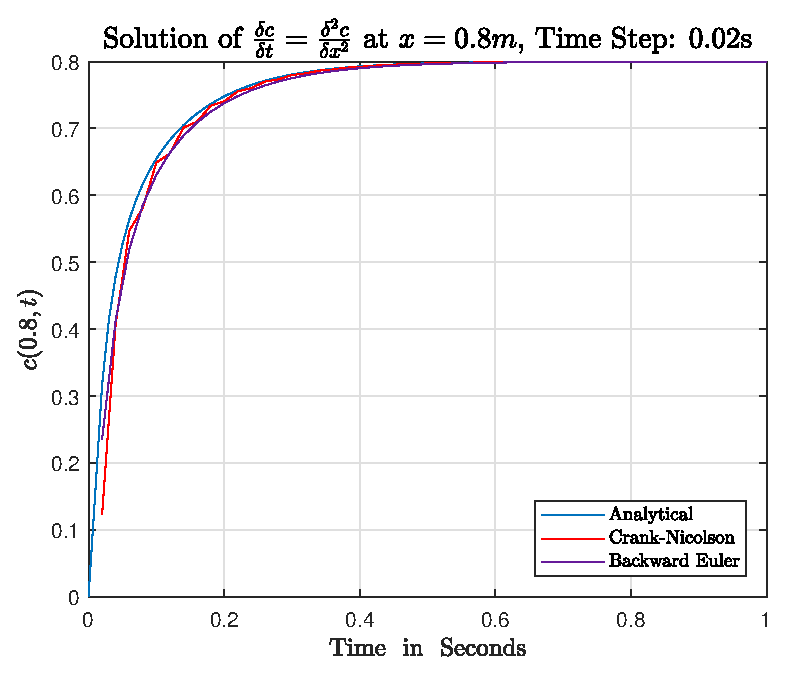
\includegraphics[width=\textwidth]{epsQ1bdt025}
            \caption[]%
            {{\small Time Step of 0.02s}}    
            \label{fig:q1b025}
        \end{subfigure}
        \caption[ Comparison of Time Stepping Schemes ]
        {\small Comparison of Crank-Nicolson and Backward Euler Time Stepping Schemes, $dx = 0.1$} 
        \label{fig:q1b}
\end{figure}

The formula for Backward Euler and Crank-Nicolson are given by equations \eqref{eq:back} and \eqref{eq:crank} respectively. It can seen that the Backward Euler method is a first order approximation and so truncates terms $O(\Delta t)^2$ and higher. The Crank-Nicolson method is a second order approximation which is can be seen by rewriting $t^{n+1}$ as $t^{n+1} = t^n+\Delta t$ in equation \eqref{eq:crank}. Therefore the error is of order  $O(\Delta t)^3$ and higher which explains why it matches the analytical solution more closely in Figures \ref{fig:q1b10} and \ref{fig:q1b025} .
\begin{subequations}
\begin{align}
u^{n+1} &= u^n + f(t^{n+1},u^{n+1})\Delta t \label{eq:back} \\ 
u^{n+1} &= u^n + \frac{1}{2}[f(t^n,u^n) + f(t^{n+1},u^{n+1})]\Delta t \label{eq:crank} 
\end{align}
\end{subequations}

\FloatBarrier
\subsection{Investigating the L2 Norm}

The L2 norm is the error of the FEM solution compared to the analytical solution. As the $L_2$ Norm is investigating the error in the  spatial domain the time step had to be very small to make the time error, discussed previously, insignificant. As a result only low resolution meshes could be tested to keep computing time reasonable. Equation \eqref{eq:l2norm1} shows how the exact solution $CE(x)$ is approximated by the FEM solution $C(x)$ with an additional higher order terms truncated. For linear basis functions the lowest order truncated term, n,  is $n = 2$, and similarly for quadratic basis functions $n = 3$.

\begin{equation} \label{eq:l2norm1}
CE(x) = C(x) + O(h^n)
\end{equation}

The error $E(x)$ is $CE(x) - C(x)$ and by rewriting the higher $O(h^n)$ as $Gh^n$, where $G$ is a constant, equation \eqref{eq:l2norm1} can be written as equation \eqref{eq:l2normgrad}. It can be seen that as the error converges with increasing mesh resolution the gradient of the a logarithmic plot of these should be $n$. 


\begin{equation} \label{eq:l2normgrad}
log(E(x)) = log(G) + n*log(h)
\end{equation}

The $L_2$ norm was calculated for mesh sizes of 5 to 12 elements and plotted as shown in Figures \ref{fig:q1l2o1} and \ref{fig:q1l2o2} for linear and quadratic basis functions respectively. The gradients were computed to be -1.97 and -2.88 for linear and quadratic plots respectively. This shows that the $L_2$ norm is converging as the gradients match the expected $n$ values of the truncated terms. 


\begin{figure}[ht] 
        \centering
        \begin{subfigure}[b]{0.475\textwidth}
            \centering
            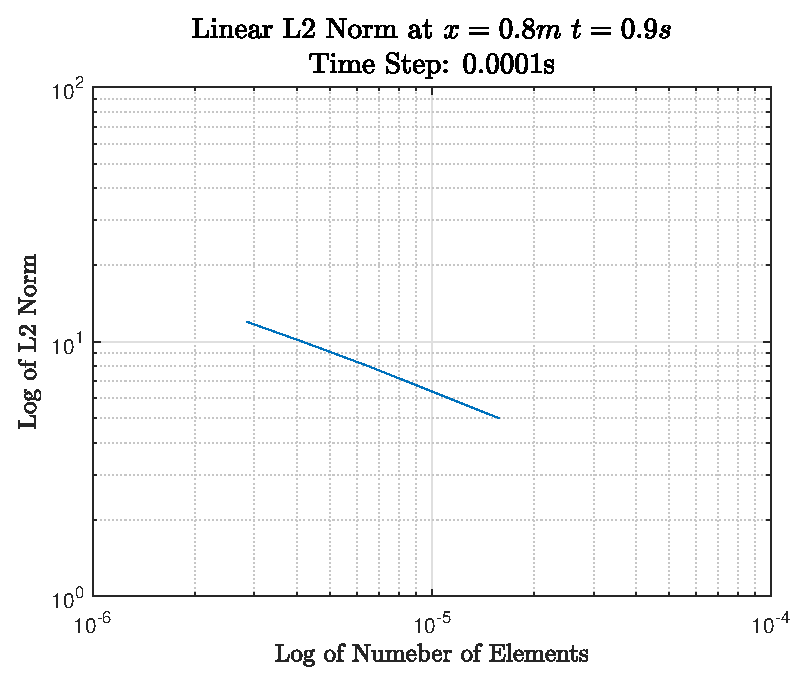
\includegraphics[width=\textwidth]{epsQ1L2O1}
            \caption[]%
            {{\small Gradient = -1.97 }}    
            \label{fig:q1l2o1}
        \end{subfigure}
        \hfill
        \begin{subfigure}[b]{0.475\textwidth}  
            \centering 
            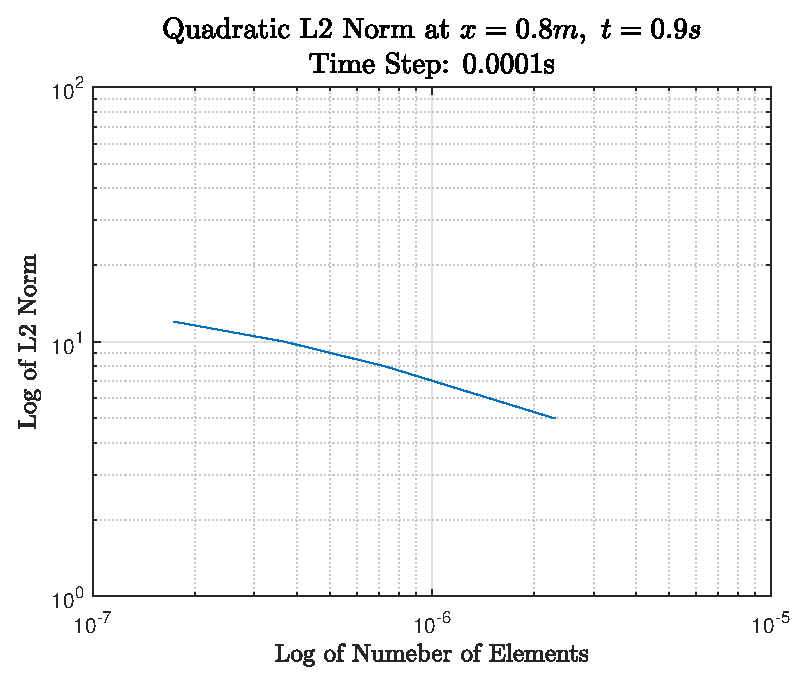
\includegraphics[width=\textwidth]{epsQ1L2O2}
            \caption[]%
            {{\small Gradient = -2.88}}    
            \label{fig:q1l2o2}
        \end{subfigure}
        \caption[ Convergence of L2 Norm for Linear and Quadratic Basis Functions.]
        {\small Comparison of Error Convergence for Linear and Quadratic Basis Functions.} 
        \label{fig:q1bl2grad}
\end{figure}
\pagebreak


\section{Part 2: Modeling and Simulation Results}

\subsection{Question 1}

\subsubsection{Introduction of Problem}

The code developed in Part 1 was used to model heat transfer through skin. The skin is split into layers and the heat transfer through the first three layers was investigated. The spatial domain, $x$, is defined by Figure \ref{fig:skinlayers} with the following boundary positions:
\begin{equation*}
 B = 0.01 \ , \ \ D = 0.005 \ , \ \ E  =  0.00166667.
\end{equation*}

\begin{figure}[!h]  %nrcVrc Figure
	\centering
	\includegraphics[width=.75\textwidth]{SkinStructure.png}
    \caption{Layout of Skin Layers and the $x$ Domain \cite{cw2}.}\label{fig:skinlayers}
\end{figure}

The material properties are not consistent between layers and are defined in Table \ref{table:defparams}.
\FloatBarrier
\begin{table}[!h]
\centering %Set parameters table
\ra{1.3}
\begin{tabular}{@{}cccc@{}}\toprule
 \textbf{Parameter}  & \textbf{Epidermis} &  \textbf{Dermis} & \textbf{Sub-cutaneous} \\
\midrule
$ k$ & 25  &  40  & 20 \\
$G$ & 0  & 0.0375  & 0.0375 \\
$\rho$ & 1200  &  1200  &  1200 \\
$c$ & 3300 & 3300  & 3300 \\
$\rho_b$ & -  & 1060  & 1060 \\
$c_b$ & -  & 3770  &  3770\\
$T_b$  & - & 310.15  &  310.15  \\
\bottomrule
\end{tabular}
\caption{Material Properties of Skin at Each Layer.}
\label{table:defparams}
\end{table}
\FloatBarrier

The governing equation of heat transfer over the $x$ domain is given by equation \eqref{eq:goveqn} where parameters  were defined in Table \ref{table:defparams}. When compared to the standard form of the transient diffusion-reaction equation the value of the coefficients $D$, $\lambda$ and $f$ can be written as equations \eqref{eq:coeffd}, \eqref{eq:coefflambda} and \eqref{eq:coefff} respectively. 

\begin{equation} \label{eq:goveqn}
\frac{\partial T}{\partial t}    = \bigg(\frac{k}{\rho c} \bigg)\frac{\partial^2 T}{\partial x^2} - \bigg(\frac{G \rho_b c_b}{\rho c}\bigg)T + \bigg(\frac{G \rho_b c_b}{\rho c}\bigg)T_b
\end{equation}

\begin{subequations}
\begin{align}
D &= \frac{k}{\rho c} \label{eq:coeffd} \\ 
\lambda &= \frac{G \rho_b c_b}{\rho c} \label{eq:coefflambda} \\  
f &=  \frac{G \rho_b c_b}{\rho c}T_b \label{eq:coefff}
\end{align}
\end{subequations}

The solver created for question one was used to solve equation \eqref{eq:goveqn} over the time domain $t = 0s \ \text{to} \ t = 50s$. Initially the problem was modeled with zero blood flow, i.e $G = 0$. The model set-up as per Table \ref{table:q1setup} with the following boundary and initial conditions. 

\begin{subequations}\label{eq:q2conds}
\begin{align}
T(x,0) &= 310.15K \label{eq:q2ic} \\ 
T(x = 0,t) &= 310.15K \label{eq:q2lhbc} \\  
T(x = B, t)&=  393.15K \label{eq:q2rhbc}
\end{align}
\end{subequations}


\begin{table}[!h]
\centering %Set parameters table
\ra{1.3}
\begin{tabular}{@{}rl@{}}\toprule
 \textbf{Parameter}  & \textbf{Value}  \\
\midrule
No. Elements  & 100  \\
Time Step ($\delta t$) & 0.005   \\
Stepping Scheme & Backward Euler  \\
Basis Function Order & 2 (Quadratic)  \\
\midrule
$D$ (Epiderm., Derm., Sub-cut.) &  $6.31e-06, 1.01e-05, 5.05e-6$ \\
$\lambda$ & 0 \\
$f$  &0 \\
$\frac{D \delta t}{\delta x^2}$  (Epiderm., Derm., Sub-cut.)  & 6.31, 10.1, 5.05 \\
\bottomrule
\end{tabular}
\caption{Material Properties of Skin at Each Layer.}
\label{table:q1setup}
\end{table}

\clearpage
\FloatBarrier
\subsubsection{ Temperature Profiles}
From the result a three dimensional plot of temperature variation in space and time was created to visualise the overall system as shown in Figure \ref{fig:surf1}. 
\FloatBarrier
\begin{figure}[!h]  %nrcVrc Figure
	\centering
	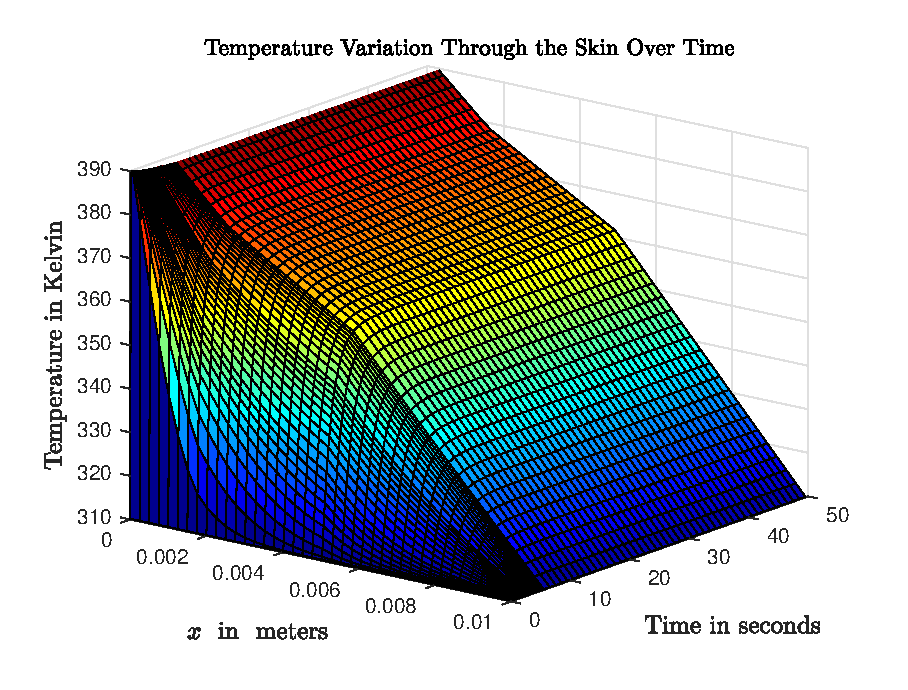
\includegraphics[width=.75\textwidth]{ManualSurf.eps}
    \caption{Temperature Profiles in Space and Time. }\label{fig:surf1}
\end{figure}
\FloatBarrier

Several of these temperature profiles at points time have been plotted in more detail in Figure \ref{fig:q21profs}. It can be seen  that over the 50s period the temperature profile rises from the initial condition of 310.15K to a steady state profile which is linear within the individual layers. The gradients in each layer are linked to the thermal conductivity, $k$, of the tissue in that layer. For example, for the steady state solution at $t = 50s$, the temperature gradient in the Sub-cutaneous region is double that of the Dermis region at $10,200 \ K/m$ compared to $5,100 \ K/m$. The inverse is true of the thermal conductivity, $k$ with $k = \ 20 W/m.K$ in the Sub-cutaneous and $k = 40 \ W/m.K$ in the Dermis. As heat transfer occurs at a greater rate in materials of higher thermal conductivity, the temperature variation through the material is reduced, and so the temperature profile is flatter explaining the lower temperature gradient in the Dermis region.\\

The flow of thermal energy from the skin surface inward is also evident. As the internal boundary condition is the same as the initial condition the profile is over time is driven by the external boundary which is significantly hotter at 393.15K compared to 310.15 for the initial and internal boundary conditions. This means temperatures rise much faster at the external boundary. For example the after 0.5s the temperature has risen 52\% of the difference to the steady state at the Epidermis-Dermis boundary but only 13\% at the Dermis to Sub-cutaneous boundary as the energy has not conducted through yet. This also explains why the gradient within each layer decreases decreases with depth before the steady state is approached giving the curved profiles. Conversely there is very little change in temperature over time near the internal boundary as the boundary condition is the same as the initial condition.
\FloatBarrier

\begin{figure}[!h]  %nrcVrc Figure
	\centering
	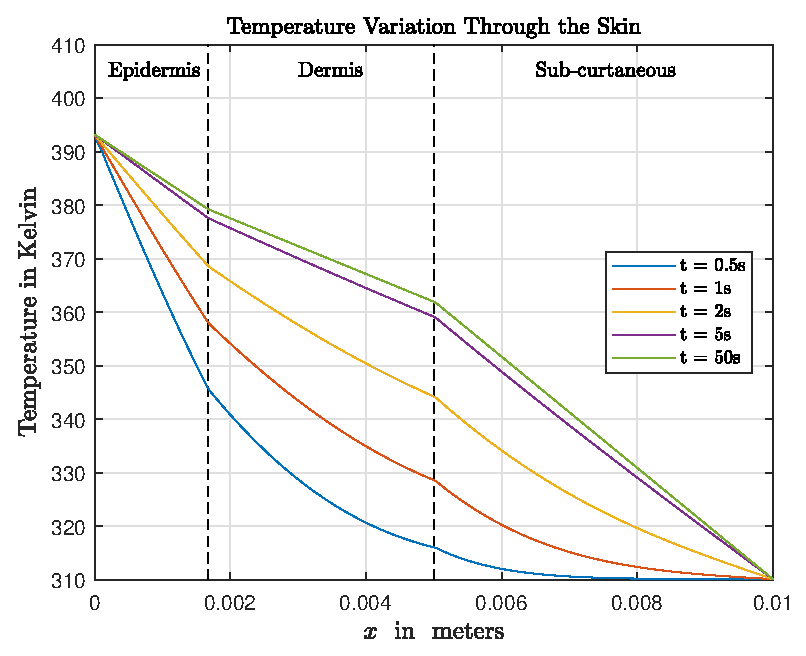
\includegraphics[width=.75\textwidth]{epsQ21TempXT}
    \caption{Temperature Profiles at Various Points in Time. }\label{fig:q21profs}
\end{figure}
\FloatBarrier
Figure \ref{fig:q21time} shows the variation in temperature at $x = 0.002m$ and $x = 0.005m$ over the time domain. It is again clear that the temperature fastest at $x = 0.002m$ as it is closest to the external boundary. It can also be seen that the steady state solution has been approached before $t = 50s$. The profiles become very flat after $t = 20s$ and so the problem is no longer a truly transient after this steady state solution has been reached. At $x = 0.002m$ the temperature after $t=21.35s$ is the calculated to be the same as the temperature at $t=50s$  to 8 significant figures i.e T = 377.5372K. As such adaptive time stepping would be particularly efficient for this problem to increase the time step at steady state

\FloatBarrier

\begin{figure}[!h]  %nrcVrc Figure
	\centering
	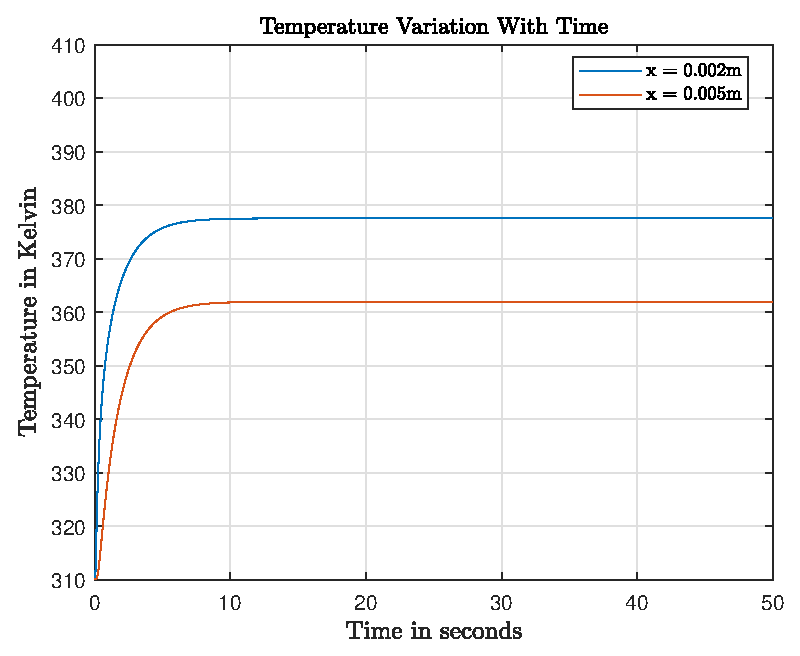
\includegraphics[width=.75\textwidth]{epsTimePlot}
    \caption{Temperature Variation With Time Showing Steady State Solution is Approached. }\label{fig:q21time}
\end{figure}

\FloatBarrier




\subsubsection{Evaluating Tissue Damage}

Tissue damage can occur when tissue is at a high temperature for an extended period of time. This can be numerically evaluated using equation \ref{eq:burn}. The equation is evaluated at one point in the skin and if $\Gamma > 1$ a second-degree burn will occur at that point. 

\begin{equation} \label{eq:burn}
\Gamma = \int^{t}_{t_{burn}} 2 \times 10^{98} \exp{\bigg(- \frac{12017}{(T - 273.15)}\bigg)} dt
\end{equation}

The function EvalGamma.m, available in Appendix \ref{ap:EvalGamma}, was written to evaluate this integral using Matlab software's trapezium rule integration function. For the conditions given by equation \eqref{eq:q2conds} the calculated result was $\Gamma = 2.01e+50$. Therefore second degree burns were expected to occur. 

\clearpage
\FloatBarrier
\subsection{Question 2}


The function EvalGamma.m shown returned the value of $\Gamma$ at the Epidermis-Dermis boundary for a given external boundary condition, $T(x=0, t) $. From Part 2 Question 1 it was known that a boundary condition of $T(x=0, t) = 393.15$K results in   $\Gamma >> 1$. Furthermore, as the temperature which burning occurs is $T_{burn} = 317.15$K, a boundary condition of $T(x=0, t) = 316$K will produce the result  $\Gamma < 1$. \\



A algorithm was made to calculate the value of $T(0,t)$ to within 0.5K which would produce a result of $\Gamma = 1$. The script is called FindBC.m and is shown in Appendix \ref{ap:FindBC}. The process followed to find the boundary condition is described by the flow chart in Figure \ref{fig:BCflowchart}. The initial high and low temperature bounds were set at $T(0, t) = 394$K and $T(0, t) = 316$K to give results for $\Gamma$ above and below the target value of $\Gamma = 1$. The process took 8 iterations to give the temperature range of $T(0,t) = 328.5\text{K} \ \text{to} \ 328.8$K. \\

\begin{table}[!h]
\centering %Set parameters table
\ra{1.3}
\begin{tabular}{@{}ccccl@{}}\toprule
 Iteration  & $T_{high}$ (K) & $T_{low}$ (K) &  $T_{av}$ (K) & $\Gamma (T_{av}) $ \\
\midrule
1 \   & 394 & 316  &  355  &  2.05e+29\\
2 \   & 355 & 316  &  335.5  & 4.75e+09 \\
3 \   & 335.5 & 316  &  325.75  &  1.13e-05 \\
4 \   & 335.5 & 325.75  & 330.63  & 825 \\
5 \   & 330.63 & 325.75  &  328.19  & 0.138 \\
6 \   & 330.63 & 328.19  & 329.41  &  11.58\\
7 \   & 329.41 & 328.19  &  328.80  & 1.2892  \\
8 \   & \textbf{328.80} & 328.19  &  \textbf{328.49}  & 0.4233  \\
\midrule
Result & 328.8 & 328.5 & \textbf{328.6} & \textbf{0.74}\\
\bottomrule
\end{tabular}
\caption{Result of Boundary Condition Finding Algorithm at Each Iteration With No  Blood Flow.}
\label{table:findbc}
\end{table}

 It was difficult to design a more efficient algorithm such as the shooting method to determine the boundary condition due to the high degree of non-linearity between $\Gamma$ and $T(0,t)$. The result at each iteration of the algorithm is shown in Table \ref{table:findbc} and gives insight into how the algorithm arrived at the solution of $T(0, t) =T$. Also the temperature variation with time at the Dermis-Epidermis boundary has been plotted at selected iterations in Figure \ref{fig:q22profs}. The boundary condition for each interval plotted in Figure \ref{fig:q22profs} is given by the $T_{av}$ for the corresponding iteration in Table \ref{table:findbc}. \\

\begin{figure}[t]  %nrcVrc Figure
	\centering
	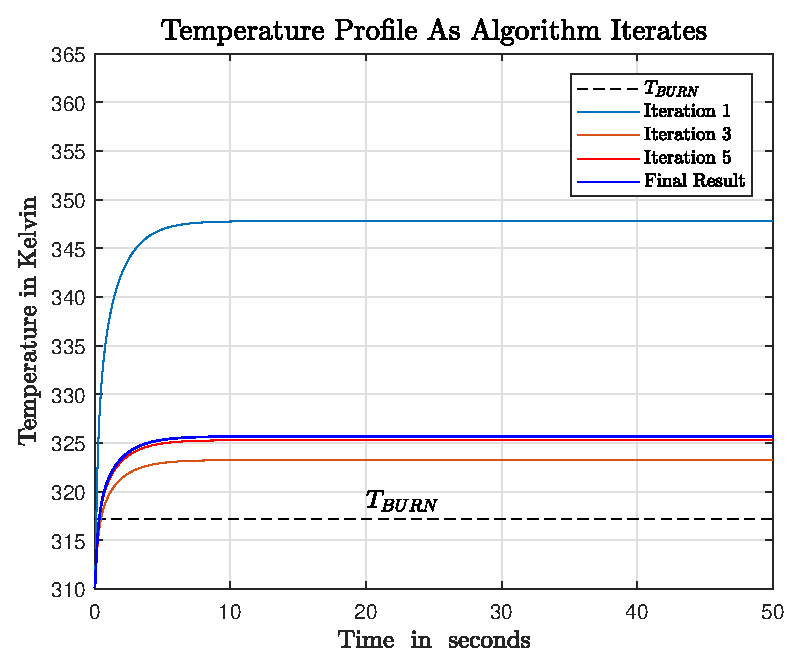
\includegraphics[width=.75\textwidth]{epsQ22BCTempProfs}
    \caption{Temperature Profiles As Algorithm Converges on $\Gamma = 1$.}\label{fig:q22profs}
\end{figure}
\FloatBarrier
As in previous question Figure \ref{fig:q22profs} shows the steady state solution is approached very quickly and so the majority of burning occurs at steady state conditions. For this reason Backward Euler time stepping scheme was used as it meant a large time step could be used, thus converging on the steady state solution quicker. The sacrifice of greater error in the more transient region at the start would not contribute as much to the calculation of $\Gamma$ as no much time is spent in this region and at the start where the error is greatest the temperature is less that $T_{burn}$ and so is not included in the calculation of $\Gamma$. This was important as calculating for several iterations becomes computationally expensive.


\begin{figure}[ht]  %nrcVrc Figure
	\centering
	\includegraphics[width=.6\textwidth]{FindBC.pdf}
    \caption{Flow Chart Showing The Process Followed by The BCFinder.m Script}\label{fig:BCflowchart}
\end{figure}

\FloatBarrier
\subsection{Question 3}

Question 2 was repeated but with blood flow, $G$, included which took the values given in Table \ref{table:defparams}. The effect of blood flow is shown in Figure \ref{fig:q3profs} where it has been compared to the no blood flow case for the conditions given by equation \eqref{eq:q2conds}. It can be seen that the blood flow reduces temperature across the profile absorbing thermal energy from the system as the entire system is at a higher temperature than the blood. The temperature reduction is greatest at the steady state which as discussed has the greatest bearing on whether a second degree burn occurs. 


\begin{figure}[!h]  %nrcVrc Figure
	\centering
	\includegraphics[width=.75\textwidth]{epsQ3Profiles}
    \caption{Temperature Profiles at Various Points in Time, With and Without Blood Flow. Conditions Given in Table 3 and Equation 9.}\label{fig:q3profs}
\end{figure}
\FloatBarrier


 The result of the iterative process to find the hottest boundary condition at which a second degree burn does not occur ( $\Gamma  = 1$) is given in Table \ref{table:q3bc}. The temperature was found to be $T = 329.3$K compared to $T = 328.6$K with no blood flow. The temperature profiles over time for the \mbox{$T(0,t) = 329.3$K} solution have been plotted in Figure \ref{fig:q3profs2}. The effect of blood flow is greatly reduced compared to Figure \ref{fig:q3profs} as the steady state temperature profile is much closer to the blood temperature. The effectiveness of the blood as a heat sink is reduced greatly by its absence in the Epidermis layer as the skin temperature is highest here. The large temperature differential would allow greater transfer of heat. Close to the inside boundary, where the blood temperature and boundary condition are the same, the blood is ineffective at transferring away heat. The 0.7K boundary condition temperature rise is significant however as it is greater than the 0.5K range required so it was worth adding blood flow to the model. 

\begin{figure}[!h]  %nrcVrc Figure
	\centering
	\includegraphics[width=.75\textwidth]{epsQ3Profiles2}
    \caption{Temperature Profiles at Various Points in Time for $\Gamma = 1$ Conditions. }\label{fig:q3profs2}
\end{figure}
\FloatBarrier

\begin{table}[!h]
\centering %Set parameters table
\ra{1.3}
\begin{tabular}{@{}ccccl@{}}\toprule
 Iteration  & $T_{high}$ (K) & $T_{low}$ (K) &  $T_{av}$ (K) & $\Gamma (T_{av}) $ \\
\midrule
1 \   & 394 & 316  &  355  &  2.32e+28\\
2 \   & 355 & 316  &  335.5  & 6.36e+08 \\
3 \   & 335.5 & 316  &  325.75  &  2.12e-06 \\
4 \   & 335.5 & 325.75  & 330.63  & 126 \\
5 \   & 330.63 & 325.75  &  328.19  &   0.023 \\
6 \   & 330.63 & 328.19  & 329.41  &  1.85\\
7 \   & 329.41 & 328.19  &  328.80  & 0.211  \\
8 \   & \textbf{329.41} &  328.80  &  \textbf{329.10}  &  0.629  \\
\midrule
Result &329.4 & 329.1 & \textbf{329.3} & \textbf{1.08}\\
\bottomrule
\end{tabular}
\caption{Result of Boundary Condition Finding Algorithm at Each Iteration When Blood Flow is Included.}
\label{table:q3bc}
\end{table}

\clearpage


\FloatBarrier
\subsection{Question 4}

There many assumptions in the model which need to be addressed. 

\begin{enumerate}
\item{\textbf{Constant Blood Flow}}
\begin{itemize}
\item{\textit{Assumption} -Vasodilation has not been modeled. This is where blood flow, $G$, increases as skin tissue temperature rises above normal levels. The effect is to transport away more heat from the tissue meaning a higher temperature external boundary condition at which a second degree burn occurs.}
\item{\textit{Improvement} - If the relationship between blood flow and body temperature was known this effect could have been accounted for by recalculating $G$ based on the previous temperature at each node for every nth time step. By only recalculating every nth time step, such as n = 10,  a more realistic result could be found with only a small increase in computing time. This does assume no lag in the blood flow temperature response which is also inaccurate.}
\end{itemize}
\item{\textbf{Constant Material Parameters}}
\begin{itemize}
\item{\textit{Assumption} - Material parameters do not change with temperature. This assumption is not acceptable for cases where there is burning at the external boundary. The burning is would significantly affect the thermal and physical properties of the skin and the model would be particularly non-representative of reality in the region near the burnt skin surface.  }
\end{itemize}
\item{\textbf{Dirichlet Boundary Conditions}}
\begin{itemize}
\item{\textit{Assumption} - Temperature at both boundaries is constant. This is a fair assumption for the external boundary which is potentially subjected to a constant temperature source. The assumption is not accurate for the internal boundary condition as the temperature past the Sub-cutaneous region will rise as the thermal energy dissipates through the skin. However for the specific problem of checking for second degree burn at the Epidermis-Dermis boundary this is an acceptable assumption. This is because the internal boundary is much further away from the Epidermis-Dermis boundary that than the external boundary and so has much less influence over the temperature at this point. }
\item{\textit{Improvement} It could be advantageous to used a mixed boundary condition at the internal boundary so that flux may leave the internal boundary if temperatures exceed the 310.15K body temperature. }
\end{itemize}
\end{enumerate}

\begin{thebibliography}{9}
%%Last name, First Initial, Year published. Title. Publisher, Volume, Page(s).
%% HARVARD REFERENCE STYLE:
%%Brunner, F.H., 1949. Synthetic gasoline from natural gas. Industrial and engineering chemistry, 41(11), pp.2511-2515.
%

\bibitem{errors} 
Cellier, F.E.; Kofman, E., 2006. 
\textit{Continuous System Simulation.}\\
Springer

\bibitem{cw2} 
Cookson. A, 2018. 
\textit{Coursework 2.}\\
University of Bath
\end{thebibliography}

%%\\\\\\\\\\\\\\\\\\\\\\\\\\\\\\\\\      APPENDICIES         \\\\\\\\\\\\\\\\\\\\\\\\\\\\\\\\\\\\\\\\\\\\\\\\\\\\\\\\\\\\\%%%%%%%%
\FloatBarrier
\begin{appendices}





\section{Flow Chart of FEM Solver}

\begin{figure}[ht]  %nrcVrc Figure
	\centering
	\includegraphics[width=.88\textwidth]{TRDS_FLOW.pdf}
    \caption{Flow Chart Showing The Process Followed by The FEM solver TransReactDiffSolver.m}\label{fig:TRDS}
\end{figure}
\clearpage
%%AAAAAAAAAAAAAAAAAAAAAAAAAA%%%%%%%


\section{Transient Diffusion Reaction Solver}\label{ap:TRDS}

\begin{lstlisting}
function [Ct_matrix] = TransReactDiffSolver(mesh, dt, Tend, theta, BC, NBC, IC, order, SaveRate)
%% This function solves the transient diffusion-reation equation using the
%Finite Element Method
% Inputs:
%   mesh -  1D mesh containing mesh information (structure)
%   dt -    Timestep
%   Tend -  Function will calculate solution until this time is reached
%   theta - Method of timestepping (0 for forward Euler, 0.5 for
%           Crank-Niclson, 1 for backward Euler)
%   BC -    Dirichlet Boundary Conditions (structure)
%   NBC -   Neumann Boundary Conditions (matix)
%   IC -    Initial Condition (vector)
%   order - The order of Basis Functions (1 for Linear, 2 for Quadratic)
%   SaveRate - Number of timesteps between outputted results

%% Set Number of Guass points
Ngp = order+1;

%% Initalise time
Tvec = 0:dt:Tend;

%% Initial condition, t = 0
Cnext = IC;
Ct_matrix(:,1) = Cnext;



%% Iterate through remaining timesteps
for i = 2:length(Tvec)
    
    %Set most previous time step solution to current solution
    Ccurrent = Cnext;
    % Calculate Source, Stiffness and Mass Global Matrices at this timestep
    F = SourceVectorGen(mesh, Ngp, order);  %Source
    K = GlobalStiffnessMatrixGen(mesh, Ngp, order);  %Stiffness
    M = GlobalMassMatrixGen(mesh, Ngp, order);  %Mass
    GM = M + theta*dt*K;
    tempM = (M - (1-theta)*dt*K);
    GVec = tempM*Ccurrent;
    %Add Source Vector to Global Vector
    GVec = GVec + dt*(theta*F + (1-theta)*F);
    %Add Neumann BC to source Vector
    GVec = GVec + dt*(theta*NBC(:,i-1) + (1-theta)*NBC(:,i));
    
    %Apply Boundary Conditions
    [GM, GVec] = ApplyBCs(BC, GM, GVec, mesh.ne, order);
    %Calculate next C solution vector
    Cnext = GM\GVec;
    
    
    %% Save Every 5th timestep in matlab matrix
    if mod(i-1,SaveRate) == 0
        Ct_matrix(:,((i-1)/SaveRate)+1) = Cnext;
    end
    
end
end

\end{lstlisting}
\pagebreak
%%%%%%%%%%%%%%%%%%%%%%%%%%%%%%%%%%%%%%%      SOURCE      %%%%%%%
\subsection{Source Vector Generator}\label{ap:SVGen}

\begin{lstlisting}
function [F] = SourceVectorGen(mesh, Ngp, order)
%Generates source vector
% Inputs:
%   mesh -  1D mesh containing mesh parameters (structure)
%   Ngp - Number of Gauss points for the Gauss scheme
%   order - The order of Basis Functions (1 for Linear, 2 for Quadratic)

ne = mesh.ne;   %Number of elements

%% Initalise Gloabal Source Vector F
F = zeros(order*ne+1,1);     %Initialise Source Vector

%% Add in the Constant and Linear Element Vectors and Add to F
for eID = 1:ne
    
    %Caluculate Source Local Element Vectors
    LocalSourceVector = SourceLEVec(mesh, eID, Ngp, order);
    
    %Find start and end index for the element
    StIdx = eID + (eID-1)*(order-1);
    EndIdx = StIdx + order;
    
    %Add Local Source Vector into Global Source Vector at correct location
    F(StIdx:EndIdx) = F(StIdx:EndIdx) + LocalSourceVector;
end

\end{lstlisting}
\pagebreak

\subsubsection{Local Source Vector}\label{ap:SLEV}

\begin{lstlisting}
function [LocalSourceVec] = SourceLEVec(mesh, eID, Ngp, order)
% Returns the Local Element Vector (LEVec) for the source term
%
% Inputs:
%   mesh - 1D mesh containing mesh parameters (structure)
%   Ngp - Number of Gauss points for the Gauss scheme 
%   eID - The elements unique index
%   order - The order of Basis Functions (1 for Linear, 2 for Quadratic)

gq = CreateGQScheme(Ngp);
LocalSourceVec = zeros(order+1,1); %Initialize local element matrix

%% Create local element, evaluate using Guassian Quadrature
for row = 1:(order+1)
    for i = 1:Ngp
        %Get the value of the current Gauss point
        xipt = gq.xipts(i);
        %Get source coefficient
        SourceCoeff = EvalField(mesh, mesh.fvec, eID,xipt,order);
        %Get the psi value common for the current row
        psi_row = EvalBasis(row-1,xipt,order);
        %Add each integration into loval vector
        LocalSourceVec(row,1) = LocalSourceVec(row,1) + SourceCoeff*psi_row;
    end
end

%% Multiply by J and f
J =mesh.elem(eID).J;        %Get Jacobi for the element
LocalSourceVec = J*LocalSourceVec;

end

\end{lstlisting}
\pagebreak

%%%%%%%%%%%%%%%%%%%%%%%%%%%%%%%%%%%%%%%%   STIFFNESS %%%%%%%%
\subsection{Global Stiffness Matrix}\label{ap:Stiff}
\begin{lstlisting}
function [F] = SourceVectorGen(mesh, Ngp, order)
%Generates source vector
% Inputs:
%   mesh -  1D mesh containing mesh parameters (structure)
%   Ngp - Number of Gauss points for the Gauss scheme
%   order - The order of Basis Functions (1 for Linear, 2 for Quadratic)

ne = mesh.ne;   %Number of elements

%% Initalise Gloabal Source Vector F
F = zeros(order*ne+1,1);     %Initialise Source Vector

%% Add in the Constant and Linear Element Vectors and Add to F
for eID = 1:ne
    
    %Caluculate Source Local Element Vectors
    LocalSourceVector = SourceLEVec(mesh, eID, Ngp, order);
    
    %Find start and end index for the element
    StIdx = eID + (eID-1)*(order-1);
    EndIdx = StIdx + order;
    
    %Add Local Source Vector into Global Source Vector at correct location
    F(StIdx:EndIdx) = F(StIdx:EndIdx) + LocalSourceVector;
end

\end{lstlisting}
\pagebreak


\subsubsection{Diffusion Local Element Matrix}\label{ap:DiffLEM}

\begin{lstlisting}
function [DiffLEM] = DiffLEM(msh, Ngp, eID, order)
%% Returns the Local Element Diffusion Matrix
% Inputs:
%   mesh - 1D mesh containing mesh parameters (structure)
%   Ngp - Number of Gauss points for the Gauss scheme 
%   eID - The elements unique index
%   order - The order of Basis Functions (1 for Linear, 2 for Quadratic)

gq = CreateGQScheme(Ngp);
DiffLEM = zeros(order+1); %Initialize local element matrix

%% Evaluate local element matrix cells using Guassian Quadrature
for row = 1:(order+1)
    for col = 1:(order+1)
        for i = 1:Ngp
            %Get the value of the current Gauss point
            xipt = gq.xipts(i);
            %Evaluate Material Coefficient
            MatCoeff = EvalField(msh,msh.DCvec, eID,xipt,order);
            %Evaluate Gradient common for the current row
            row_grad = EvalBasisGrad(row-1,xipt,order);
            %Evaluate Gradient common for the current column
            col_grad = EvalBasisGrad(col-1,xipt,order);
            %Add integral for each Gauss point to the current cell
            DiffLEM(row,col) = DiffLEM(row,col) + MatCoeff*col_grad*row_grad;
        end
    end
end

%%Divide by the Jacobian
J = msh.elem(eID).J;
DiffLEM = DiffLEM/J;
end
\end{lstlisting}
\pagebreak



\subsubsection{Reaction Local Element Matrix}\label{ap:ReactLEM}

\begin{lstlisting}
function [ReactLEM] = ReactLEM(mesh, Ngp, eID, order)
%% Returns the Local Element Reaction Matrix
% Inputs:
%   mesh - 1D mesh containing mesh parameters (structure)
%   Ngp - Number of Gauss points for the Gauss scheme 
%   eID - The elements unique index
%   order - The order of Basis Functions (1 for Linear, 2 for Quadratic)

%% Initiate Gauss Scheme and Rection LEM (Local Element Matrix)
gq = CreateGQScheme(Ngp);   %Gauss Scheme
ReactLEM = zeros(order+1);  %Initialize local element matrix

%% Evaluate local element matrix cells using Guassian Quadrature
for row = 1:(order+1)
    for col = 1:(order+1)
        for i = 1:Ngp
            %Get the value of the current Gauss point
            xipt = gq.xipts(i);
            %Get matierial coefficient
            MatCoeff = EvalField(mesh,mesh.RCvec, eID,xipt,order);
            %Get the psi value common for the current row
            psi_row = EvalBasis(row-1,xipt,order);
            %Get the psi value common for the current column
            psi_col = EvalBasis(col-1,xipt,order);
            %Add integral for each Gauss point to the current cell
            ReactLEM(row,col) = ReactLEM(row,col) + MatCoeff*psi_col*psi_row;
        end
    end
end

%% Multiple by the Jacobian
J = mesh.elem(eID).J;   %Jacobian 
ReactLEM = J*ReactLEM;  %Reaction LEM solution
end

\end{lstlisting}
\pagebreak

%%%%%%%%%%%%%%%%%%%%%%%%%%%%%%%%%%%%%%%%%     MASS MASS MASS

\subsection{Global Mass Matrix}\label{ap:Mass}

\begin{lstlisting}
function [GlobalMass] = GlobalMassMatrixGen(mesh, Ngp, order)
%%Returns the Global mass matrix by iterating through elements and adding
% the local element matrices for diffusion and reaction into the global
% matrix in the correct position
% Inputs:
%   mesh -  1D mesh containing mesh parameters (structure)
%   Ngp - Number of Gauss points for the Gauss scheme
%   order - The order of Basis Functions (1 for Linear, 2 for Quadratic)


%% Initiate Global Matrix
ne = mesh.ne;       %Number of Elements
GlobalMass = zeros((order*ne +1),(order*ne +1));  
%% Loop over Elements and Assemble Local Element Matrices into Global Matrix
for eID = 1:ne
        
    %Local Element Matrix is the Diffusion subtract the Linear Reation
    MassLocal = MassLEM(mesh, Ngp, eID, order);
    
    %Find start and end index for the element
    StIdx = eID + (eID-1)*(order-1);
    EndIdx = StIdx + order;
    
    %Add Local Element Matrix into the correct location within the Global Matrix
    GlobalMass(StIdx:EndIdx, StIdx:EndIdx) = GlobalMass(StIdx:EndIdx, StIdx:EndIdx)...
                                            + MassLocal;
end
\end{lstlisting}
\pagebreak

\subsubsection{Mass Local Element Matrix}\label{ap:MassElem}

\begin{lstlisting}
function [MassLEM] = MassLEM(mesh, Ngp, eID, order)
%% Returns the Local Element Mass Matrix
% Inputs:
%   mesh - 1D mesh containing mesh parameters (structure)
%   Ngp - Number of Gauss points for the Gauss scheme
%   eID - The elements unique index
%   order - The order of Basis Functions (1 for Linear, 2 for Quadratic)

%% Initialise Guass Scheme and Local Element Matrix
gq = CreateGQScheme(Ngp); %Create the Gauss scheme
MassLEM = zeros(order+1); %Initialize local element matrix

%% Evaluate local element matrix cells using Guassian Quadrature
for row = 1:(order+1)   %Iterate over rows
    
    for col = 1:(order+1)   %Iterate over the columns in the row
        
        %Use Guassian Quadrature to intergrate the eqn for the cell
        for i = 1:Ngp
            %Get the value of the current Gauss point
            xipt = gq.xipts(i);
            %Get the psi value common for the row
            psi_row = EvalBasis(row-1,xipt,order);
            %Get the psi value common for the column
            psi_col = EvalBasis(col-1,xipt,order);
            %Add integral for each Gauss point to the current cell
            MassLEM(row,col) = MassLEM(row,col) + psi_col*psi_row;
            
        end
    end
end

%% Multiply by Jacobian
J = mesh.elem(eID).J;    %Jaocbian
MassLEM = J*MassLEM;    %Local element matrix solution

end
\end{lstlisting}

\pagebreak
\subsection{Apply Boundary Conditions}\label{ap:ApplyBC}

\begin{lstlisting}
function [GlobalMatrix, F] = ApplyBCs(BC, GlobalMatrix, F, ne, order)
% Applies boundary conditions to F and Global Matrix as appropriate
% for the specified boundary condition
%
%Inputs:
%BC - Structure which contains the following:
%       BC(1) - Holds data for minimum x boundary
%       BC(2) - Holds data for maximum x boundary
%       BC().type - Type of boundary condition: "neumann", "dirichlet" or
%                   "none" (must be a lower case string)
%       BC().value - Value of the boundary condition (float or int)
%
%GlobalMatrix - formation of local element matrices (NxN matrix)
%F - Source Vector (size Nx1 vector)

%Note - This has been re-used for Transient and so Neumann Boundary no
%       can not be evaluated by this function

%% If user inputted character arrays change these to strings
BC(1).type = string(BC(1).type);
BC(2).type = string(BC(2).type);

%% Solve xmin Boundary Condition 
if BC(1).type == "none" %No action needed if no boundary condition
    % pass 
    
elseif BC(1).type == "dirichlet"  %solve for a dirichlet BC
    
    %set all first row elements to 0 except first element  
    GlobalMatrix(1,:) = [1, zeros(1,ne*order)];   
    %set first element of the source vector to the xmin BC value
    F(1) = BC(1).value;
end

%% Solve xmax Boundary Condition
if BC(2).type == "none" %No action needed if no boundary condition
    % pass
    
elseif BC(2).type == "dirichlet"  %solve for dirichlet BC
    
    %set all end row elements to 0 except last element 
    GlobalMatrix(end,:) = [zeros(1,ne*order), 1];
    %set last element of the source vector to the xmax BC value
    F(end) = BC(2).value;
end

\end{lstlisting}
\pagebreak

\section{Gaussian Quadrature Scheme}\label{ap:LaplaceElem}

\begin{lstlisting}
function [ gq ] = CreateGQScheme(N)
%CreateGQScheme Creates GQ Scheme of order N
%   Creates and initialises a data structure
gq.npts = N;
if (N > 0) && (N < 6)
    %order of quadrature scheme i.e. %number of Gauss points
    gq.gsw = zeros(N,1); %array of Gauss weights
    gq.xipts = zeros(N,1); %array of Gauss points
    switch N
        case 1
            gq.gsw(1) = 2;
            gq.xipts(1) = 0;
        case 2
            gq.gsw(1) = 1;
            gq.gsw(2) = 1;
            gq.xipts(1) = -sqrt(1/3);
            gq.xipts(2) = sqrt(1/3);
        case 3
            gq.gsw(1) = 5/9;
            gq.gsw(2) = 8/9;
            gq.gsw(3) = 5/9;
            gq.xipts(1) = -sqrt(3/5);
            gq.xipts(2) = sqrt(0);
            gq.xipts(3) = sqrt(3/5);
        case 4
            gq.gsw(1) = (18 + sqrt(30))/36;
            gq.gsw(2) = (18 + sqrt(30))/36;
            gq.gsw(3) = (18 - sqrt(30))/36;
            gq.gsw(4) = (18 - sqrt(30))/36;
            gq.xipts(1) = sqrt((3/7)-(2/7)*sqrt(6/5));
            gq.xipts(2) = sqrt((3/7)-(2/7)*sqrt(6/5));
            gq.xipts(3) = sqrt((3/7)+(2/7)*sqrt(6/5));
            gq.xipts(4) = sqrt((3/7)+(2/7)*sqrt(6/5));
        case 5
            gq.gsw(1) = 128/225;
            gq.gsw(2) = (322 + 13*sqrt(70))/900;
            gq.gsw(3) = (322 + 13*sqrt(70))/900;
            gq.gsw(4) = (322 - 13*sqrt(70))/900;
            gq.gsw(5) = (322 - 13*sqrt(70))/900;
            gq.xipts(1) = 0;
            gq.xipts(2) = (1/3)*sqrt(5-2*sqrt(10/7));
            gq.xipts(3) = (1/3)*sqrt(5-2*sqrt(10/7));
            gq.xipts(4) = (1/3)*sqrt(5+2*sqrt(10/7));
            gq.xipts(5) = (1/3)*sqrt(5+2*sqrt(10/7));
    end
    
else
    fprintf('Invalid number of Gauss points specified');
end
end


\end{lstlisting}
\pagebreak

\section{Mesh Creating Functions}
\subsection{One Dimensional Linear Mesh Generator}\label{ap:Mesh1}

\begin{lstlisting}
function [mesh] = OneDimLinearMeshGen(xmin,xmax,Ne,order)
%%This function generates a one dimensional, equispaced, linear finite
%%element mesh, with Ne number of elements, between the points at x
%%position xmin and xmax.

mesh.ne = Ne; %set number of elements
mesh.ngn = order*Ne+1; %set number of global nodes
mesh.nvec = zeros(mesh.ngn,1); %allocate vector to store global node values
dx = (xmax - xmin)/Ne; %calculate element size

mesh.nvec = xmin:(dx/order):xmax;

switch order
    case 1 
        %loop over elements & set the element properties
        for i=1:Ne
            
            %set spatial positions of nodes
            mesh.elem(i).x(1) = xmin + (i-1)*dx;
            mesh.elem(i).x(2) = xmin + i*dx ;
            
            %set global IDs of the nodes
            mesh.elem(i).n(1) = i;
            mesh.elem(i).n(2) = i+1;
            
            %set element Jacobian based on mapping to standard element
            mesh.elem(i).J = 0.5*dx; %this is assuming standard element of -1 to 1 
        end
    case 2
          %loop over elements & set the element properties
        for i=1:Ne
            
            %set spatial positions of nodes
            mesh.elem(i).x(1) = xmin + (i-1)*dx;
            mesh.elem(i).x(2) = mesh.elem(i).x(1) + dx/2; 
            mesh.elem(i).x(3) = xmin + i*dx ;
            
            %set global IDs of the nodes
            mesh.elem(i).n(1) = i + (i-1)*(order-1);
            mesh.elem(i).n(2) = mesh.elem(i).n(1) + 1;
            mesh.elem(i).n(3) = mesh.elem(i).n(1) + 2;
            
            %set quadratic nvector to include midpoint nodes
            mesh.nvecq = xmin:dx/2:xmax;
            
            %set element Jacobian based on mapping to standard element
            mesh.elem(i).J = 0.5*dx; %this is assuming standard element of -1 to 1 
        end
        
end
\end{lstlisting}


\section{Part 1: Software Verification}
%%%%%%%%%%%%%%%%%%%%%%%%%%%%%%%%%%%%%%%%% Q1a
\subsection{Question 1a - Graph Plotting Script}\label{ap:Q1a}

\begin{lstlisting}
clear
clc

%% This script generates the figure for question 1a - Temp profiles
%Set Save Rate to limit Size of solution
SaveRate = 1; %Every time step is for good time resolution

%% Set inital parameters
order = 1;  %linear order
dt = .01;   %timestep
Tend = 1;   %run for until 1 second
Tvec = 0:dt:Tend; %Vector of timesteps
%% Create 10 element mesh
ne = 10;
mesh = OneDimLinearMeshGen(0,1,ne,order);
%% Set source constants
mesh.fvec = 0*mesh.nvec;
mesh.DCvec = ones(1,length(mesh.nvec));
mesh.RCvec = zeros(1,length(mesh.nvec));
%% Crank-Nicolson Scheme
theta = 0.5;
%% Create Boundary Condition Stucture
BC(1).type = "dirichlet";   
BC(1).value = 0;
BC(2).type = "dirichlet";
BC(2).value = 1;
NBC = zeros(length(mesh.nvec), length(Tvec));  %No Neumann Condition
%Set initial condition at t=0
IC = zeros(order*mesh.ne +1, 1);

%% Solve the Transcient Diffusion Reation equation using FEM method
SOL = TransReactDiffSolver(mesh, dt, Tend, theta, BC, NBC, IC, order, SaveRate);

sol5 = SOL(:,(.05/dt)/SaveRate + 1);        %Result at T = 0.05
sol10 = SOL(:,(.1/dt)/SaveRate + 1);       %Result at T = 0.10
sol20 = SOL(:,(.2/dt)/SaveRate + 1);       %Result at T = 0.20
sol100 = SOL(:,end);    %Result at T = 1


%% Plot FEM reults for linear basis functions:
figure()
plot(mesh.nvec, sol5(1:end), '--r','HandleVisibility','off')
hold on
plot(mesh.nvec, sol10(1:end), '--', 'color', [1 0.5 1],'HandleVisibility','off')
hold on
plot(mesh.nvec, sol20(1:end), '--', 'color', [0 0.5 0.5],'HandleVisibility','off')
hold on
plot(mesh.nvec, sol100(1:end), '--b','HandleVisibility','off')
hold on


%% Plot analytical solution:
%High resolution for analytical solution
Xvec = 0:0.001:Tend;
S5 = zeros(length(Xvec),1);
S10 = zeros(length(Xvec),1);
S20 = zeros(length(Xvec),1);
S100 = zeros(length(Xvec),1);

for i = 1:length(Xvec)
    S5(i) = TransientAnalyticSoln(Xvec(i), 0.05);
    S10(i) = TransientAnalyticSoln(Xvec(i), 0.1);
    S20(i) = TransientAnalyticSoln(Xvec(i), 0.2);
    S100(i) = TransientAnalyticSoln(Xvec(i), 0.9);
end
%Plotting the Analytical Results:
plot(Xvec, S5, '-r', 'HandleVisibility','on')
hold on
plot(Xvec, S10, '-', 'color',  [1 0.5 1], 'HandleVisibility','on')
hold on
plot(Xvec, S20, '-', 'color', [0 0.5 0.5], 'HandleVisibility','on')
hold on
plot(Xvec, S100, '-b', 'HandleVisibility','on')

%% Format the figure
title('Solution of $\frac{\delta c}{\delta t} = \frac{ \delta^2 c}{\delta x^2}$ Using Linear Basis Funcitons', 'interpreter' ,'latex', 'FontSize', 14)
lgd = legend({'t = 0.05', 't = 0.10', 't = 0.20', 't = 1'},'Location', 'northwest', 'interpreter', 'latex');
lgd.Title.String = '-- \ -- FEM \ , --- Analytical';
xlabel('$x$ \ in \ Metres','interpreter','latex', 'FontSize', 12);
ylabel('$c(x)$', 'interpreter','latex', 'FontSize', 12);
grid on
%% Saving Linear Basis Function Figure
%print -depsc \Users\xav_m\OneDrive\Documents\XAVI\University\Final_Year\Systems_Mod\Modeling_CW2\Report\Figures\epsQ1a

%% Now repeat for order 2 (quadratic)
order  = 2;
ne = 5;
mesh = OneDimLinearMeshGen(0,1,ne,order);
%Set coefficient vectors
mesh.fvec = 0*mesh.nvec;
mesh.DCvec = ones(1,length(mesh.nvec));
mesh.RCvec = zeros(1,length(mesh.nvec));
%Set initial condition at t=0
IC = zeros(order*mesh.ne +1, 1);
%% Solve the Transcient Diffusion Reation equation using FEM method
SOLQ = TransReactDiffSolver(mesh, dt, Tend, theta, BC, NBC, IC, order, SaveRate);

sol5Q = SOLQ(:,(.05/dt)/SaveRate + 1);        %Result at T = 0.05
sol10Q = SOLQ(:,(.1/dt)/SaveRate + 1);       %Result at T = 0.10
sol20Q = SOLQ(:,(.2/dt)/SaveRate + 1);       %Result at T = 0.20
sol100Q = SOLQ(:,end);    %Result at T = 1

%% Plot FEM reults for linear basis functions:
figure()
plot(mesh.nvec, sol5Q, '--r','HandleVisibility','off')
hold on
plot(mesh.nvec, sol10Q, '--', 'color', [1 0.5 1],'HandleVisibility','off')
hold on
plot(mesh.nvec, sol20Q, '--', 'color', [0 0.5 0.5],'HandleVisibility','off')
hold on
plot(mesh.nvec, sol100Q, '--b','HandleVisibility','off')
hold on


%Plotting the Analytical Results:
plot(Xvec, S5, '-r', 'HandleVisibility','on')
hold on
plot(Xvec, S10, '-', 'color',  [1 0.5 1], 'HandleVisibility','on')
hold on
plot(Xvec, S20, '-', 'color', [0 0.5 0.5], 'HandleVisibility','on')
hold on
plot(Xvec, S100, '-b', 'HandleVisibility','on')
%% Format the quadratic figure
title('Solution of $\frac{\delta c}{\delta t} = \frac{ \delta^2 c}{\delta x^2}$ Using Quadratic Basis Funcitons', 'interpreter' ,'latex', 'FontSize', 14)
lgd = legend({'t = 0.05', 't = 0.10', 't = 0.20', 't = 1'},'Location', 'northwest', 'interpreter', 'latex');
lgd.Title.String = '-- \ -- FEM \ , --- Analytical';
xlabel('$x$ \ in \ Metres','interpreter','latex', 'FontSize', 12);
ylabel('$c(x)$', 'interpreter','latex', 'FontSize', 12);
grid on
%% Saving Linear Basis Function Figure
%print -depsc \Users\xav_m\OneDrive\Documents\XAVI\University\Final_Year\Systems_Mod\Modeling_CW2\Report\Figures\epsQ1aQuad


\end{lstlisting}


\pagebreak
%%%%%%%%%%%%%%%%%%%%%%%%%%%%%%%%%%%%%%%%% Q1a
\subsection{Question 1b - Graph Plotting Script}\label{ap:Q1b}

\begin{lstlisting}

clear
clc

%% This script generates the figure for question 1b - T at x = 0.8m

%Set Save Rate to limit Size of solution
SaveRate = 1; %Every time step is for good time resolution

%Solve the FEM solution:
%% Set inital parameters
order = 2;  %quadratic order
dt = 0.01;   %timestep
Tend = 1;   %run for until 1 second
Tvec = 0:dt:Tend; %Vector of timesteps
%% Create 10 element mesh
ne = 10;
mesh = OneDimLinearMeshGen(0,1,ne,order);
%% Set source constants
mesh.fvec = 0*mesh.nvec;    %No source
mesh.DCvec = ones(1,length(mesh.nvec)); %D = 1 everywhere
mesh.RCvec = zeros(1,length(mesh.nvec)); % No reaction
%% Time Stepping Scheme
theta = 0.5;    % Crank-Nicolson Scheme
%% Create Boundary Condition Stucture
BC(1).type = "dirichlet";   
BC(1).value = 0;
BC(2).type = "dirichlet";
BC(2).value = 1;
NBC = zeros(length(mesh.nvec), length(Tvec));  %No Neumann Condition
%Set initial condition at t=0
IC = zeros(order*mesh.ne +1, 1);



%% Solve the Transcient Diffusion Reation equation using FEM method
SOL = TransReactDiffSolver(mesh, dt, Tend, theta, BC, NBC, IC, order, SaveRate);


%% Solve using the Analytical Solution:
TvecAn = 0:0.01:Tend;
C80_Analytic = zeros(length(TvecAn), 1);
for i = 1:length(TvecAn)
    C80_Analytic(i) = TransientAnalyticSoln(0.8, TvecAn(i));
end

%% Plot how temperature varies at x = 0.8
Tvec = 0:dt*SaveRate:Tend;  %Set time vector for analytical plot
C80 = SOL(8*order+1, :);  %Crank-Nicolson at x = 0.80
fig = figure();
plot(TvecAn, C80_Analytic, '-')     %Plot Analytic Solution
hold on
plot(Tvec(2:end),C80(2:end), '-r')     %Plot Crank-Nicolson

%% Format the Figure
title({'Solution of $\frac{\delta c}{\delta t} = \frac{ \delta^2 c}{\delta x^2}$ at $x = 0.8m$, Time Step: 0.01s'}, 'interpreter' ,'latex', 'FontSize', 14)
lgd = legend({'Analytical', 'Crank-Nicolson'},'Location', 'southeast', 'interpreter', 'latex');
lgd.Title.String = '-- \ -- FEM \ , --- Analytical';
xlabel('Time \ in \ Seconds','interpreter','latex', 'FontSize', 12);
ylabel('$c(0.8,t)$', 'interpreter','latex', 'FontSize', 12);
ylim([0 0.9])
grid on
%% Saving Linear Basis Time Stepping Scheme Figure
%print -depsc \Users\xav_m\OneDrive\Documents\XAVI\University\Final_Year\Systems_Mod\Modeling_CW2\Report\Figures\epsQ1b

%Creat and save a zoomed plot
figzoom = gcf;
ylim auto
xlim([0.05 0.052])
%% Saving Zoomed Figure
%print -depsc \Users\xav_m\OneDrive\Documents\XAVI\University\Final_Year\Systems_Mod\Modeling_CW2\Report\Figures\epsQ1bZoom

\end{lstlisting}

\pagebreak
\subsection{Question 1 Extra - Investigating Time Stepping Schemes}\label{ap:L2}
\begin{lstlisting}
%% Script to compare time stepping schemes
clear
clc
color1 = [0.4 0.1 0.6]; %Color for plotting
%% Set inital parameters
order = 1;  %linear order
dt = 0.1;   %timestep
Tend = 1;   %run for until 1 second
Tvec = 0:dt:Tend; %Vector of timesteps
SaveRate = 1;   %Save every time ttep to see oscilations
%% Create 10 element mesh
ne = 10;
mesh = OneDimLinearMeshGen(0,1,ne,order);
%% Set source constants
mesh.fvec = 0*mesh.nvec;    %No source
mesh.DCvec = ones(1,length(mesh.nvec)); %D = 1 everywhere
mesh.RCvec = zeros(1,length(mesh.nvec)); % No reaction
%% Time Stepping Scheme
theta = 0.5;    % Crank-Nicolson Scheme
%% Create Boundary Condition Stucture
BC(1).type = "dirichlet";   
BC(1).value = 0;
BC(2).type = "dirichlet";
BC(2).value = 1;
NBC = zeros(length(mesh.nvec), length(Tvec));  %No Neumann Condition
%Set initial condition at t=0
IC = zeros(order*mesh.ne +1, 1);

%% Solve Using Crank-Nicolson Time Stepping Scheme
SOL_CN = TransReactDiffSolver(mesh, dt, Tend, theta, BC, NBC, IC, order, SaveRate);

%% Solve using Backward Euler Timestepping
theta = 1;  %Backward Euler scheme
SOL_BE = TransReactDiffSolver(mesh, dt, Tend, theta, BC, NBC, IC, order, SaveRate);

%% Solve using the Analytical Solution
TvecAn = 0:0.01:Tend;
C80_Analytic = zeros(length(TvecAn), 1);
for i = 1:length(TvecAn)
    C80_Analytic(i) = TransientAnalyticSoln(0.8, TvecAn(i));
end
    
%% Plot how temperature varies at x = 0.8
Tvec = 0:dt:Tend;
C80_CN = SOL_CN(8*order+1, :);  %Crank-Nicolson at x = 0.80
C80_BE = SOL_BE(8*order+1, :);  %Backward Euler at x = 0.80
figure()
plot(TvecAn, C80_Analytic, '-')     %Plot Analytic Solution
hold on
plot(Tvec(2:SaveRate:end),C80_CN(2:end), '-*r')     %Plot Crank-Nicolson
hold on
plot(Tvec(2:SaveRate:end),C80_BE(2:end), '-x', 'color', color1)     %Plot Backward Euler

%% Format the Figure
title({'Solution of $\frac{\delta c}{\delta t} = \frac{ \delta^2 c}{\delta x^2}$ at $x = 0.8m$, Time Step: 0.1s'}, 'interpreter' ,'latex', 'FontSize', 14)
legend({'Analytical', 'Crank-Nicolson', 'Backward Euler'},'Location', 'southeast', 'interpreter', 'latex');
xlabel('Time \ in \ Seconds','interpreter','latex', 'FontSize', 12);
ylabel('$c(0.8,t)$', 'interpreter','latex', 'FontSize', 12);
grid on
%% Saving 0.1s Time Step Figure
%print -depsc \Users\xav_m\OneDrive\Documents\XAVI\University\Final_Year\Systems_Mod\Modeling_CW2\Report\Figures\epsQ1bdt05


%% %%%%  Repeat with smaller timestep 
dt = .02;   %New timestep
Tvec = 0:dt:Tend; %Vector of timesteps
NBC = zeros(length(mesh.nvec), length(Tvec));  %No Neumann Condition
%% Solve Using Crank-Nicolson Time Stepping Scheme
theta = 0.5;    %Crank-Nicolson Scheme
SOL_CN = TransReactDiffSolver(mesh, dt, Tend, theta, BC, NBC, IC, order, SaveRate);

%% Solve using Backward Euler Timestepping
theta = 1;  %Backward Euler scheme
SOL_BE = TransReactDiffSolver(mesh, dt, Tend, theta, BC, NBC, IC, order, SaveRate);

%% Plot how temperature varies at x = 0.8
Tvec = 0:dt:Tend;   %Time Vector for FEM solutions
C80_CN = SOL_CN(8*order+1, :);  %Crank-Nicolson at x = 0.80
C80_BE = SOL_BE(8*order+1, :);  %Backward Euler at x = 0.80
figure()
plot(TvecAn, C80_Analytic, '-')     %Plot Analytic Solution
hold on
plot(Tvec(2:SaveRate:end),C80_CN(2:end), '-r')     %Plot Crank-Nicolson
hold on
plot(Tvec(2:SaveRate:end),C80_BE(2:end), '-', 'color', color1)     %Plot Backward Euler

%% Format the Figure
title({'Solution of $\frac{\delta c}{\delta t} = \frac{ \delta^2 c}{\delta x^2}$ at $x = 0.8m$, Time Step: 0.02s'}, 'interpreter' ,'latex', 'FontSize', 14)
legend({'Analytical', 'Crank-Nicolson', 'Backward Euler'},'Location', 'southeast', 'interpreter', 'latex');
xlabel('Time \ in \ Seconds','interpreter','latex', 'FontSize', 12);
ylabel('$c(0.8,t)$', 'interpreter','latex', 'FontSize', 12);
ylim([0 0.9])
grid on
%% Saving 0.02s Time Step Figure
%print -depsc \Users\xav_m\OneDrive\Documents\XAVI\University\Final_Year\Systems_Mod\Modeling_CW2\Report\Figures\epsQ1bdt025


\end{lstlisting}


\pagebreak
%%%%%%%%%%%% \\\\\\\\\\\\\\\\\\\\\\\\\\\\\\\\\\\\\\\\\\\\\\\\\\\\\\\\\\\\\\\\\\\\\\\\\\\\\\\\\\\\\\\\   L2 L2 L2 L2 
\subsection{Question 1 Extra - Investigating L2 Norm}\label{ap:L2}


\subsubsection{L2 Norm Script}\label{ap:L2Script}

\begin{lstlisting}
%% Script to evaluate the L2 norm for the Transcient solver for quadratic
% and linear cases
clear
clc
%Set Save Rate to limit Size of solution
SaveRate = 1; %Every time step is for good time resolution

%Quad Order
order = 2;  %order
dt = .0001;  % timestep
Tend = 1;   %run for until 1 second
Tvec = 0:dt:Tend; %Vector of timesteps
%Crank Scheme
theta = 1;
%% Create Boundary Condition Stucture
BC(1).type = "dirichlet";
BC(1).value = 0;
BC(2).type = "dirichlet";
BC(2).value = 1;

%% Caulculate L2 norm for different mesh resolutions
ne = [5, 8, 10, 12];    %The mesh sizes to used
for i = 1:length(ne)
    mesh = OneDimLinearMeshGen(0,1,ne(i),order);    %Create the mesh
    %% Set source constants
    mesh.fvec = 0*mesh.nvec;
    mesh.DCvec = ones(1,length(mesh.nvec));
    mesh.RCvec = 0*mesh.nvec;
    %Set Neumann Condition
    NBC = zeros(length(mesh.nvec), length(Tvec));  %No Neumann Condition
    %Set initial condition at t=0
    IC = zeros(order*mesh.ne +1, 1);
    %Calculate Solution
    SOL = TransReactDiffSolver(mesh, dt, Tend, theta, BC, IC, order, SaveRate);
    %Get solution at x = 0.9m
    C_FEM = SOL(:,(0.9/(dt*SaveRate))+1);
    %Calculate L2 norm
    L2(i) = L2norm(mesh, C_FEM, order, 0.9);
    %Calculate Logs
    L2log(i) = log(L2(i));
    nelog(i) = log(ne(i));
end
%% Calculate line of best fit
fitvars = polyfit(nelog, L2log, 1);
%Get the gradient of the line
grad = fitvars(1)
%Plot log log graph
figure()
loglog(L2,ne)

%% Format the Figure
title({'Quadratic L2 Norm at $x = 0.8m, \ t = 0.9s$','Time Step: 0.0001s'}, 'interpreter' ,'latex', 'FontSize', 14)
xlabel('Log of Numeber of Elements','interpreter','latex', 'FontSize', 12);
ylabel('Log of L2 Norm', 'interpreter','latex', 'FontSize', 12);
grid on
%% Saving Linear Basis Time Stepping Scheme Figure
%print -depsc \Users\xav_m\OneDrive\Documents\XAVI\University\Final_Year\Systems_Mod\Modeling_CW2\Report\Figures\epsQ1L2O2

%% Repeating for Order 1
order = 1;  %linear order
%% Caulculate L2 norm for different mesh resolutions
ne = [5, 8, 10, 12];    %The mesh sizes to used
for i = 1:length(ne)
    mesh = OneDimLinearMeshGen(0,1,ne(i),order);    %Create the mesh
    %% Set source constants
    mesh.fvec = 0*mesh.nvec;
    mesh.DCvec = ones(1,length(mesh.nvec));
    mesh.RCvec = zeros(1,length(mesh.nvec));
    %Set Neumann Condition
    NBC = zeros(length(mesh.nvec), length(Tvec));  %No Neumann Condition
    IC = zeros(order*mesh.ne +1, 1);    %Set initial condition at t=0
    %Calculate Solution
    SOL = TransReactDiffSolver(mesh, dt, Tend, theta, BC, IC, order, SaveRate);
    %Get solution at x = 0.9m
    C_FEM = SOL(:,(0.9/(dt*SaveRate))+1);
    %Calculate L2 norm
    L2(i) = L2norm(mesh, C_FEM, order, 0.9);
    %Calculate logs
    L2log(i) = log(L2(i));
    nelog(i) = log(ne(i));
end
%% Calculate line of best fit
fitvars2 = polyfit(nelog, L2log, 1);
%Get the gradient of the line
grad2 = fitvars2(1)
%Plot log log graph
figure()
loglog(L2,ne)

%% Format the Figure
title({'Linear L2 Norm at $x = 0.8m \ t = 0.9s$', 'Time Step: 0.0001s'}, 'interpreter' ,'latex', 'FontSize', 14)
xlabel('Log of Numeber of Elements','interpreter','latex', 'FontSize', 12);
ylabel('Log of L2 Norm', 'interpreter','latex', 'FontSize', 12);
grid on
%% Saving Linear Basis Time Stepping Scheme Figure
%print -depsc \Users\xav_m\OneDrive\Documents\XAVI\University\Final_Year\Systems_Mod\Modeling_CW2\Report\Figures\epsQ1L2O1

\end{lstlisting}
\pagebreak

\subsubsection{L2 Norm Function}\label{ap:L2Function}

\begin{lstlisting}
function [L2norm] = L2norm(mesh, C_FEM, order, t)
%% Calculates the L2 norm error for a vector
% Inputs:
%   mesh - A mesh containing various information (structure)
%   C_FEM - The numerical solution (vector)
%   order - The order of Basis Functions (1 for Linear, 2 for Quadratic)
%   t - The time at which the L2 norm is being calculated for (seconds)


%% Set up Gauss Scheme
Ngp = order+2; %Number of gauss ponts
gq = CreateGQScheme(Ngp);   %Creat Gauss Scheme
Nel = mesh.ne; %Number of elements
%% Initialise error to 0
error = 0;

%% Integrate using Gaussian Quadrature
switch order
    case 1  %% Solve for Linear Basis Functions
        for eID = 1:Nel
            
            %Get Jacobian for the element
            J = mesh.elem(eID).J;
            %x values element nodes
            x0 = mesh.elem(eID).x(1);
            x1 = mesh.elem(eID).x(2);
            %c values at element nodes
            c0 = C_FEM(eID); 
            c1 = C_FEM(eID+1); 
            
            %Loop through gauss points for the element
            for i2 = 1:Ngp
                %Get Gaussian weight
                wi = gq.gsw(i2);
                %Evaluate Basis functions at the Gauss Point
                psi0 = EvalBasis(0,gq.xipts(i2),order);
                psi1 = EvalBasis(1,gq.xipts(i2),order);
                %Evaluate x and c
                x = x0*psi0 + x1*psi1;
                C = c0*psi0 + c1*psi1;
                %Get exact solution
                Ce = TransientAnalyticSoln(x,t);
                %Add error at this Gauss point to the cumilating error
                error = error + J*wi*(Ce - C)^2;
            end
        end
        
    case 2  %% Solve for Quadratic Basis Functions
        for eID = 1:Nel
            
            %Get Jacobian for the element
            J = mesh.elem(eID).J;
            %x values element nodes
            x0 = mesh.elem(eID).x(1);
            x1 = mesh.elem(eID).x(2);
            x2 = mesh.elem(eID).x(3);
            %c values at element nodes
            c0 = C_FEM(mesh.elem(eID).n(1)); 
            c1 = C_FEM(mesh.elem(eID).n(2));
            c2 = C_FEM(mesh.elem(eID).n(3));
            
            %% Loop through gauss points for the element
            for i2 = 1:Ngp
                %Get Gaussian weight
                wi = gq.gsw(i2);
                %Evaluate Basis functions at the Gauss Point
                psi0 = EvalBasis(0,gq.xipts(i2),order);
                psi1 = EvalBasis(1,gq.xipts(i2),order);
                psi2 = EvalBasis(2,gq.xipts(i2),order);
                %Evaluate x and c
                x = x0*psi0 + x1*psi1 + x2*psi2;
                C = c0*psi0 + c1*psi1 + c2*psi2;
                %Get exact solution
                Ce = TransientAnalyticSoln(x,t);
                
                %Add error at this Gauss point to the cumilating error
                error = error + J*wi*(Ce - C)^2;
            end
        end
end

%% Square root the error to get the L2 norm
L2norm = sqrt(error);

end
\end{lstlisting}
\pagebreak

\section{Part 2: Modelling and Simulation Results}

\subsection{Adding Material Properties into Mesh}

\subsubsection{Skin Material Property Structure Generator}
\begin{lstlisting}
function [skin] = getSkinProperties(bloodflow)
%%%% Setting properties through the skin for the specific case defined
%%%% in part 2 of Coursework 2. 

%% Set Sub-Cutaneous Properties
skin.SubCut.start = 0.005;  %Start point (m)
skin.SubCut.end = 0.01;     %End point (m)
skin.SubCut.k = 20;     %Thermal Conductivity (W / m K)
skin.SubCut.G = 0.0375; %Blood Flow Rate(m^3/s)
skin.SubCut.c = 3300;   %Specific Heat Capacity of tissue (J/kgK)
skin.SubCut.rho = 1200;     %Density of the tissue (kg/m^3)
skin.SubCut.rhoB = 1060;    %Density of blood (kg/m^3)
skin.SubCut.cB = 3770;  %Specific Heat Capacity of blood (J/kgK)
skin.SubCut.TB = 310.15;    %Temperature of blood (K)


%% Set Dermis Properties
skin.dermis.start = 15/9000;  %Start point (m)
skin.dermis.end = 0.005;      %End point (m)
skin.dermis.k = 40;     %Thermal Conductivity (W / m K)
skin.dermis.G = 0.0375; %Blood Flow Rate(m^3/s)
skin.dermis.c = 3300;   %Specific Heat Capacity of tissue (J/kgK)
skin.dermis.rho = 1200;     %Density of the tissue (kg/m^3)
skin.dermis.rhoB = 1060;    %Density of blood (kg/m^3)
skin.dermis.cB = 3770;  %Specific Heat Capacity of blood (J/kgK)
skin.dermis.TB = 310.15;    %Temperature of blood (K)

%% Set epidermis Properties
skin.epidermis.start = 0;       %Start point (m)
skin.epidermis.end = 15/9000;   %End point (m)
skin.epidermis.k = 25;      %Thermal Conductivity (W / m K)
skin.epidermis.G = 0;       %Blood Flow Rate(m^3/s)
skin.epidermis.c = 3300;   %Specific Heat Capacity of tissue (J/kgK)
skin.epidermis.rho = 1200;     %Density of the tissue (kg/m^3)
skin.epidermis.rhoB = 0;    %Density of blood (kg/m^3)
skin.epidermis.cB = 0;  %Specific Heat Capacity of blood (J/kgK)
skin.epidermis.TB = 0;    %Temperature of blood (K)

%% Set all bloodflow to zero for no bloodflow condition
if bloodflow == false
    skin.SubCut.G = 0;
    skin.dermis.G = 0;
end
       
\end{lstlisting}
\clearpage
\subsubsection{Add Material Coefficients To Mesh Function}
\begin{lstlisting}
function [mesh] = setMatCoeffVectors(mesh, bloodflow, order)
%% This function sets the Material Coefficients for Diffusion, Reaction
%   and source. The skin properties for each layer are found using
%   getSkinProperties.m and then coefficients are set at each node
% Inputs:
%   mesh -  1D mesh containing mesh information (structure)
%   bloodflow - logical to indicate if there is bloodflow
%               (takes the value 'true' or 'false')

%% Initialise the vectors for coefficent

mesh.DCvec = zeros(order*mesh.ne,1);      %Diffusion Coefficient vector
mesh.RCvec = zeros(order*mesh.ne,1);      %Reaction Coefficient vector
mesh.fvec = zeros(order*mesh.ne,1);       %Source Coefficient vector


%% Calculate Coefficients at each layer
%Get structure containing porperties of the skin and each layer
skin = getSkinProperties(bloodflow);

%Sub Curtaneous Coefficients
skin.SubCut.D = skin.SubCut.k / (skin.SubCut.rho * skin.SubCut.c);

skin.SubCut.lambda = -(skin.SubCut.G * skin.SubCut.rhoB * skin.SubCut.cB)/ ...
    (skin.SubCut.rho * skin.SubCut.c);

skin.SubCut.f = (-1) * skin.SubCut.lambda * skin.SubCut.TB;

%Dermis Coefficients
skin.dermis.D = skin.dermis.k / (skin.dermis.rho * skin.dermis.c);

skin.dermis.lambda = -(skin.dermis.G * skin.dermis.rhoB * skin.dermis.cB)/ ...
    (skin.dermis.rho * skin.dermis.c);

skin.dermis.f = (-1) * skin.dermis.lambda * skin.dermis.TB;

%Epiermis Coefficients
skin.epidermis.D = skin.epidermis.k / (skin.epidermis.rho * skin.epidermis.c);

skin.epidermis.lambda = -(skin.epidermis.G * skin.epidermis.rhoB * skin.epidermis.cB)/ ...
    (skin.epidermis.rho * skin.epidermis.c);

skin.epidermis.f = (-1) * skin.epidermis.lambda * skin.epidermis.TB;

%% Now cycle through nodes and set coefficients as appropiate
for i = 1:length(mesh.nvec)
    
    if mesh.nvec(i) >= skin.epidermis.start && mesh.nvec(i) <= skin.epidermis.end
        mesh.DCvec(i) = skin.epidermis.D;
        mesh.RCvec(i) = skin.epidermis.lambda;
        mesh.fvec(i) = skin.epidermis.f;
        
    elseif mesh.nvec(i) > skin.dermis.start && mesh.nvec(i) <= skin.dermis.end
        
        mesh.DCvec(i) = skin.dermis.D;
        mesh.RCvec(i) = skin.dermis.lambda;
        mesh.fvec(i) = skin.dermis.f;
        
    elseif mesh.nvec(i) > skin.SubCut.start && mesh.nvec(i) <= skin.SubCut.end
        mesh.DCvec(i) = skin.SubCut.D;
        mesh.RCvec(i) = skin.SubCut.lambda;
        mesh.fvec(i) = skin.SubCut.f ;
    else
        error('Node x position is not within the skin layers given')
    end
end
end


\end{lstlisting}
\pagebreak

\subsection{Question 1a }
\subsubsection{Graph Plotting Script}
\begin{lstlisting}
%% This script generates the result for Part 2 Question 2a
clear
clc

%Set Save Rate to limit Size of solution
SaveRate = 5; %Every fith time step is sufficient resolution


%% Set up the problem
%Create mesh
order = 2;  %quadratic order
xmin = 0;
xmax = 0.01;
Ne = 100;    % Number of elements
mesh = OneDimLinearMeshGen(xmin, xmax, Ne, order); %Create mesh

%Add Material and source coefficients to mesh
bloodflow = false; % no blood flow
mesh = setMatCoeffVectors(mesh, bloodflow, order); 

%Set time stepping properties
theta = 1;     %Backward Euler Time Stepping Scheme
dt = 0.005;     %Time step
Tend = 50;  %Run over 50s domain
Tvec = 0:dt:Tend; %Vector of timesteps
%Set Initial Condition
IC = 310.15 * ones((mesh.ne*order + 1), 1);
%% Create Boundary Condition Stucture
BC(1).type = "dirichlet";
BC(1).value = 393.15;
BC(2).type = "dirichlet";
BC(2).value = 310.15;
NBC = zeros(length(mesh.nvec), length(Tvec));  %No Neumann Condition

%SOL = TransReactDiffSolver(mesh, dt, Tend, theta, BC, NBC, IC, order, SaveRate);
%Write result to csv file to save having to re-run:
%dlmwrite('Q1aResult.csv', SOL, 'delimiter', ',', 'precision', 17);
%Read in previous result so don't have to run whilst formatting
SOL = csvread('Q1aResult.csv');

%% Plot Temperature Profiles
figure()
%Plot skin boundary and regions
%Epidermis Boundary and text
plot([15/9000 15/9000], [310 410], '--k', 'HandleVisibility', 'off')
hold on
text(0.0002, 405, 'Epidermis', 'interpreter', 'latex', 'FontSize', 10)
%Dermis Boundary and text
plot([.005 .005], [310 410], '--k', 'HandleVisibility', 'off')
hold on
text(.003, 405, 'Dermis', 'interpreter', 'latex', 'FontSize', 10)
%Sub-cutaneous Region Text
text(.0065, 405, 'Sub-curtaneous', 'interpreter', 'latex', 'FontSize', 10)

%Plot Temperature Profiles
plot(mesh.nvec, SOL(:,(0.5/dt)/5))  %Plot profile at t = 0.5s
hold on
plot(mesh.nvec, SOL(:,(1/dt)/5))    %Plot profile at t = 1s
hold on
plot(mesh.nvec, SOL(:,(2/dt)/5))    %Plot profile at t = 2s
hold on
plot(mesh.nvec, SOL(:,(5/dt)/5))    %Plot profile at t = 5s
hold on
plot(mesh.nvec, SOL(:,end))         %Plot profile at t =50s

%% Format the figure
title('Temperature Variation Through the Skin', 'interpreter', 'latex')
legend({'t = 0.5s', 't = 1s' , 't = 2s', 't = 5s', 't = 50s'}, 'interpreter', 'latex', 'location', 'east')
xlabel('$x$ \ in \ meters','interpreter','latex', 'FontSize', 12);
ylabel('Temperature in Kelvin', 'interpreter','latex', 'FontSize', 12);
ylim([310 410]);
grid on
%% Saving The Figure
%print -depsc \Users\xav_m\OneDrive\Documents\XAVI\University\Final_Year\Systems_Mod\Modeling_CW2\Report\Figures\epsQ21TempXT

%% Plotting variation of T at single depth point with time
figure()
plot(0:.005*SaveRate:Tend, SOL(41,:))
hold on
plot(0:.005*SaveRate:Tend, SOL(101,:))
%% Format the figure
title('Temperature Variation With Time', 'interpreter', 'latex')
legend({'x = 0.002m', 'x = 0.005m'}, 'interpreter', 'latex', 'location', 'best')
xlabel('Time  in  seconds','interpreter','latex', 'FontSize', 12);
ylabel('Temperature in Kelvin', 'interpreter','latex', 'FontSize', 12);
ylim([310 410]);
grid on
%print -depsc \Users\xav_m\OneDrive\Documents\XAVI\University\Final_Year\Systems_Mod\Modeling_CW2\Report\Figures\epsTimePlot

%% Create surf plot
figure()
TimeVec = 0:dt*SaveRate:Tend;
%Space out time plots to improve clarity of figure
Tidx = [1:4:41 , 47:6:101, 113:12:221 ,261:40:length(TimeVec)];
%Get X, Y and Z 
Xsurf = mesh.nvec(1:5:end);
Ysurf = TimeVec(Tidx);
Zsurf = SOL(1:5:end, Tidx)';
%Plot
surf(Xsurf , Ysurf,  Zsurf)
colormap jet
%% Format the figure
title('Temperature Variation Through the Skin Over Time', 'interpreter', 'latex')
xlabel('$x$ \ in \ meters','interpreter','latex', 'FontSize', 12);
ylabel('Time  in  seconds','interpreter','latex', 'FontSize', 12);
zlabel('Temperature in Kelvin', 'interpreter','latex', 'FontSize', 12);
%Set Limits
zlim([310 390])
ylim([0 50])
xlim([0,0.01])
% grid on
%print -depsc \Users\xav_m\OneDrive\Documents\XAVI\University\Final_Year\Systems_Mod\Modeling_CW2\Report\Figures\epsSurf1

\end{lstlisting}
\pagebreak

\subsubsection{Evaluating $\Gamma$ Function} \label{ap:EvalGamma}
\begin{lstlisting}
function [Gamma, EpiBndVec] = EvalGamma(T_x0, bloodflow)

%Set Save Rate to limit Size of solution
SaveRate = 5; %Every time step is for good time resolution

%Create the mesh
order = 1;  %Linear order
xmin = 0;
xmax = 0.01;
Ne = 100;    % Number of elements
mesh = OneDimLinearMeshGen(xmin, xmax, Ne, order); %Create mesh

%Get Material and source coefficients

mesh = setMatCoeffVectors(mesh, bloodflow, order);

%Set time stepping properties
theta = 0.5;     %Backward Euler Time Stepping Scheme
dt = 0.01;     %Time step
Tend = 50;
Tvec = 0:dt:Tend; %Vector of timesteps

%Set Initial Condition
IC = 310.15 * ones((mesh.ne*order + 1), 1);
%% Create Boundary Condition Stucture
BC(1).type = "dirichlet";
BC(1).value = T_x0;
BC(2).type = "dirichlet";
BC(2).value = 310.15;
NBC = zeros(length(mesh.nvec), length(Tvec));  %No Neumann Condition

SOL = TransReactDiffSolver(mesh, dt, Tend, theta, BC, NBC, IC, order, SaveRate);

%locate epidermis boundary
i = 1;  %start ID counter
while mesh.DCvec(i) == mesh.DCvec(i+1)
    i = i+1;
end
EpiBndID = i; %Epidermis Boundary index
EpiBndVec = SOL(EpiBndID, :);   %Epidermis Boundry Temp Profile for plots
%locate timestep where burn temperatue is reached
Tburn = 317.15;
i = 1;
%Creat logical NoBurn to deal with cases where Tburn is not exceeded
NoBurn = false; %Assume Tburn exceeded

while SOL(EpiBndID,i) < Tburn
    i = i+1;
    if i+1 > length(mesh.DCvec) %Tburn is never exceeded
        NoBurn = true;  %will use this to set gamma to zero
        i = length(mesh.DCvec)-1;   %Set to minimise integration time
        break
    end
end

BurnStID = i;

%Get Vector of temperatures after burning temp is reached
BurnVec = SOL(EpiBndID, BurnStID:end);

%Calculate gamma for each temperature in the burn vector
GammaBurnVec = zeros(1, length(BurnVec)); %Initialise
for i = 1:length(BurnVec)
    GammaBurnVec(i) = 2*10^98 *exp(-12017/(BurnVec(i)-273.15));
end

%Perform Integral including limits
Gamma = (trapz(GammaBurnVec) * dt);

%Set gamma to zero if Tburn was never exceeded
if NoBurn == true
    Gamma = 0;
end
    



\end{lstlisting}

\pagebreak
\subsection{Finding Boundary Condition Algorithm} \label{ap:FindBC}
\begin{lstlisting}

bloodflow = false;

T_low = 316;   % Know result of Gamma < 1
%[~ , TempVec(1, :)] = EvalGamma(T_low, bloodflow);

T_high = 394;   % Known result of Gamma >> 1
%[~ , TempVec(2, :)] = EvalGamma(T_high, bloodflow);

i = 1
%Average the two inital guesses to get a third guess
T_av = (T_low+T_high)/2

%% While the difference between the new guess and previous guess is
%   greater than 0.5K continue iterating toward solution og Gamma = 1
while T_high-T_low > 0.5  
    
    %[Gamma, TempVec(i+2, :)]  = EvalGamma(T_av, bloodflow)
    [Gamma, ~]  = EvalGamma(T_av, bloodflow)
    
    if Gamma > 1   %
        T_high = T_av;
    else
        T_low = T_av;
    end
    i = i+1
    T_av = (T_low + T_high)/2
    
end
% Find values of Gamma for the solution Boundary Condition for completeness
%[Gamma, TempVec(i+2, :)]  = EvalGamma(T_av, bloodflow)
[Gamma, ~]  = EvalGamma(T_av, bloodflow)

%Save to csv file for post processing data
%dlmwrite('Q22TempVec.csv', TempVec, 'delimiter', ',', 'precision', 12);

\end{lstlisting}
\clearpage
\subsection{Question 2 Graph Plotting Script}
\begin{lstlisting}
%% Script to plot the temperature profiles found at iterations
%   of the FindBC.m algorithm to show how the solution was 
%   converged upon

TempMatrix = csvread('Q22TempVec.csv');

TimeVec = linspace(0, 50, 1001);
%TimeVec = TimeVec(1:200);

%% Plot the results

figure()
plot([TimeVec(1) TimeVec(end)], [317.15, 317.15], '--k') %Plot the Tburn line
text(20, 319, '$T_{BURN}$', 'interpreter', 'latex', 'FontSize', 12)
hold on
plot(TimeVec, TempMatrix(3,:), '-' ) %Plot the low temp initial guess
hold on 
plot(TimeVec, TempMatrix(5,:), '-') %Plot the high temp initial guess
hold on
plot(TimeVec, TempMatrix(7,:), '-r') %Plot the first iteration
hold on
% plot(TimeVec, TempMatrix(8,:)) %Plot the third iteration
% hold on
plot(TimeVec, TempMatrix(end,:), '-b', 'LineWidth', 0.8) %Plot the final result

%% Format the figure
title('Temperature Profile As Algorithm Iterates', 'interpreter' ,'latex', 'FontSize', 14)
lgd = legend({'$T_{BURN}$', 'Iteration 1', 'Iteration 3','Iteration 5', 'Final Result'},'Location', 'northeast', 'interpreter', 'latex');
xlabel('Time \ in \ seconds','interpreter','latex', 'FontSize', 12);
ylabel('Temperature in Kelvin', 'interpreter','latex', 'FontSize', 12);
grid on
%Set axis limits
ylim([310 365]);
xlim([0 50]);
%% Saving The Figure
%print -depsc \Users\xav_m\OneDrive\Documents\XAVI\University\Final_Year\Systems_Mod\Modeling_CW2\Report\Figures\epsQ22BCTempProfs

\end{lstlisting}
\pagebreak


\subsection{Question 3 Graph Plotting Script}
\begin{lstlisting}
%% This script generates the graphs for Part 2 Question 3
clear
clc
%Set Save Rate to limit Size of solution
SaveRate = 5; %Every fith time step is sufficient resolution

%Create the mesh
order = 2;  %Linear order
xmin = 0;
xmax = 0.01;
Ne = 100;    % Number of elements
mesh = OneDimLinearMeshGen(xmin, xmax, Ne, order); %Create mesh

%Get Material and source coefficients
bloodflow = true; % no blood flow
mesh = setMatCoeffVectors(mesh, bloodflow, order);

%Set time stepping properties
theta = 0.5;     %Backward Euler Time Stepping Scheme
dt = 0.01;     %Time step
Tend = 50;
Tvec = 0:dt:Tend; %Vector of timesteps
%Set Initial Condition
IC = 310.15 * ones((mesh.ne*order + 1), 1);
%% Create Boundary Condition Stucture
BC(1).type = "dirichlet";
BC(1).value = 393.15;
BC(2).type = "dirichlet";
BC(2).value = 310.15;
NBC = zeros(length(mesh.nvec), length(Tvec));  %No Neumann Condition

%Get bloodflow solution
SOL = TransReactDiffSolver(mesh, dt, Tend, theta, BC, NBC, IC, order);
%Write result to csv file to save having to re-run
%dlmwrite('Q3profiles.csv', SOL, 'delimiter', ',', 'precision', 17);

%Read in blood flow solution
SOL = csvread('Q3profiles.csv');

%Read in NO blood flow solution
SOL_NoBlood = csvread('Q1aResult.csv');
figure()
%Plot skin boundaries
%Epidermis Boundary
plot([15/9000 15/9000], [310 410], '--k', 'HandleVisibility', 'off')
hold on
text(0.0002, 405, 'Epidermis', 'interpreter', 'latex', 'FontSize', 10)
%Dermis Boundary
plot([.005 .005], [310 410], '--k', 'HandleVisibility', 'off')
hold on
text(.003, 405, 'Dermis', 'interpreter', 'latex', 'FontSize', 10)
%Sub-cutaneous Region Text
text(.0065, 370, 'Sub-curtaneous', 'interpreter', 'latex', 'FontSize', 10)

%Plot Temperature Profiles Including Blood Flow
plot(mesh.nvec, SOL(:,(0.5/dt)/5), '-', 'color', [0.,0.55,0.55])  %Plot profile at t = 0.5s
hold on
plot(mesh.nvec, SOL(:,(1/dt)/5), '-b')    %Plot profile at t = 1s
hold on
plot(mesh.nvec, SOL(:,(2/dt)/5), '-m')    %Plot profile at t = 2s
hold on
plot(mesh.nvec, SOL(:,end), '-r')         %Plot profile at t =50s

%Plot Temperature Profiles For No Blood
plot(mesh.nvec, SOL_NoBlood(:,(0.5/dt)/5), '--', 'color', [0.,0.55,0.55])  %Plot profile at t = 0.5s
hold on
plot(mesh.nvec, SOL_NoBlood(:,(1/dt)/5), '--b')    %Plot profile at t = 1s
hold on
plot(mesh.nvec, SOL_NoBlood(:,(2/dt)/5), '--m')    %Plot profile at t = 2s
hold on
plot(mesh.nvec, SOL_NoBlood(:,end), '--r')         %Plot profile at t =50s

%% Format the figure
title('Temperature Variation Through the Skin', 'interpreter', 'latex')
lgd = legend({'t = 0.5s', 't = 1s' , 't = 2s',  't = 50s'}, 'interpreter', 'latex', 'location', 'best');
lgd.Title.String = '-- \ -- No Blood \ --- Blood Flow';
xlabel('$x$ \ in \ meters','interpreter','latex', 'FontSize', 12);
ylabel('Temperature in Kelvin', 'interpreter','latex', 'FontSize', 12);
ylim([310 410]);
grid on
%% Saving The Figure
print -depsc \Users\xav_m\OneDrive\Documents\XAVI\University\Final_Year\Systems_Mod\Modeling_CW2\Report\Figures\epsQ3Profiles

\end{lstlisting}
\pagebreak

\section{Unit Tests}
\subsection{Unit Test For Linear and Quadratic Reaction Local Element Matrix}
 \begin{lstlisting}
%Testing ReactLEM.m creates local reation element vector correctly

%Set up initial parameters needed for the test
%%TEST FOR LINEAR AND QUADRATIC CASES
%Create Quadratic mesh
order = 2;  %Quadratic order
xmin = 0;
xmax = 0.01;
Ne = 50;    % Number of elements
meshQ = OneDimLinearMeshGen(xmin, xmax, Ne, order); %Create mesh
%Get Material and source coefficients
bloodflow = true; % no blood flow
meshQ = setMatCoeffVectors(meshQ, bloodflow, order);

%Create Linear mesh
order = 1;  %Linear order
xmin = 0;
xmax = 0.01;
Ne = 50;    % Number of elements
meshL = OneDimLinearMeshGen(xmin, xmax, Ne, order); %Create mesh

%Get Material and source coefficients
bloodflow = true; % no blood flow
meshL = setMatCoeffVectors(meshL, bloodflow, order);


%%%%% TESTS %%%%    

%% Test 1: test symmetry of the matrix for linear mesh
% Test that this matrix is symmetric
tol = 1e-14;
eID=1; %element ID
elemat = ReactLEM(meshL, 2, eID, 1); %Calculate Linear Element Matrix

assert(abs(elemat(1,2) - elemat(2,1)) <= tol && abs(elemat(1,1) - elemat(2,2))  <= tol, ...
    'Local element matrix is not symmetric!')

%% Test 2: Repeat Test 1 for quadratic funciton
% Test that this matrix is symmetric
tol = 1e-14;
eID=1; %element ID
elemat = ReactLEM(meshQ, 3, eID, 2); %Calculate Linear Element Matrix

assert(abs(elemat(1,3) - elemat(3,1)) <= tol && abs(elemat(1,1) - elemat(3,3))  <= tol, ...
    'Local element matrix is not symmetric!')
%% Test 3: test 2 different elements of the same size produce same matrix
%Test that for two elements of an equispaced mesh, as described in the
%lectures, the element matrices calculated are the same
tol = 1e-14;
eID=1; %element ID
meshL = OneDimLinearMeshGen(0,1,6,1);
meshL.RCvec = ones(1, length(meshL.nvec)); %returns random diffusion coefficient between 0 and 4

elemat1 = ReactLEM(meshL, 2, eID, 1);	%calculate element 1 matrix

eID=2; %element ID

elemat2 = ReactLEM(meshL, 2, eID, 1); %calculate element 2 matrix

diff = elemat1 - elemat2;
diffnorm = sum(sum(diff.*diff));
assert(abs(diffnorm) <= tol)

%% Test 4: Repeat Test 3 for Quadratic Basis Functions
%Test that for two elements of an equispaced mesh, as described in the
%lectures, the element matrices calculated are the same
tol = 1e-14;
eID=1; %element ID
meshQ = OneDimLinearMeshGen(0,1,6,2);   %Quadratic mesh
meshQ.RCvec = ones(1, length(meshQ.nvec)); %returns random diffusion coefficient between 0 and 4

elemat1 = ReactLEM(meshQ, 2, eID, 2);	%calculate element 1 matrix

eID=2; %element ID

elemat2 = ReactLEM(meshQ, 2, eID, 2); %calculate element 2 matrix

diff = elemat1 - elemat2;
diffnorm = sum(sum(diff.*diff));
assert(abs(diffnorm) <= tol)

%% Test 5: test that one matrix is evaluted correctly
% % Test that element 1 of the three element mesh problem described 
% in Tutorial 3 Question 2c has the element matrix evaluated correctly
tol = 1e-14;

eID=1; %element ID
mshL = OneDimLinearMeshGen(0,1,6,2);
mshL.RCvec = ones(1, length(mshL.nvec)); %diffusion coefficient

elemat1 = ReactLEM(mshL, 2, 2, 1); %calculate element 1 matrix

elemat2 = [ (1/18), (1/36); (1/36), (1/18)];    % This is the known result
diff = elemat1 - elemat2; %calculate the difference between the two matrices
SummedDiff = sum(sum(diff)); %calculates the sum of the elements in the diff matrix
assert(abs(SummedDiff) <= tol) %Checks the error of the summed differences is below tol

%% Test 6: test main diagonal values are double antidiagonal values for linear
%basis functions
% using random inputs for number of elemnts and lambda
tol = 1e-14;
eID=1; %element ID
ne = randi([4 100], 1,1);     %sets number of elements to random integer between 4 and 100
meshL = OneDimLinearMeshGen(0,1,ne,1);
meshL.RCvec = 5*abs(rand(1,1))*ones(1, length(meshL.nvec)); %returns random diffusion coefficient between 0 and 4

elemat1 = ReactLEM(meshL, 2, eID, 1);
elem = elemat1(1,1)/elemat1(2,1); %Gets ratio between 1,1 and 2,1 elements
assert(abs(elem - 2) <= tol)     %Checks ratio is 2 within the tolerance

 \end{lstlisting}

\begin{figure}[ht]  %nrcVrc Figure
	\centering
	\includegraphics[width=.8\textwidth]{ReactTest.png}
    \caption{Screenshot Of Quadratic and Linear Reaction Local Element Matrix Test.}\label{fig:ReactTest}
\end{figure}


\end{appendices}




\end{document}

